% \iffalse meta-comment
%
% Copyright (C) \the\year by Liu Benyuan <liubenyuan@gmail.com>
% This file may be distributed and/or modified under the
% conditions of the LaTeX Project Public License, either
% version 1.2 of this license or (at your option) any later
% version. The latest version of this license is in:
%
% http://www.latex-project.org/lppl.txt
%
% and version 1.2 or later is part of all distributions of
% LaTeX version 1999/12/01 or later.
%
% \fi
% 
% \iffalse
% <package>\NeedsTeXFormat{LaTeX2e}[1999/12/01]
% <package>\ProvidesPackage{nudtpaper}
% <package>		[2009/08/12 v1.0 By Liu Benyuan <liubenyuan@gmail.com>]
%<*driver>
\ProvidesFile{nudtpaper.dtx}[2009/08/12 v1.0 NUDT]
\documentclass[11pt]{ltxdoc}
\usepackage{nudtx}
\EnableCrossrefs
\CodelineIndex
\RecordChanges
\begin{document}
  \DocInput{\jobname.dtx}
\end{document}
%</driver>
% \fi
% 
% \def\thuthesis{\textsc{Thu}\-\textsc{Thesis}}
% \def\nudtpaper{\textsc{Nudt}\-\textsc{Paper}}
% 
% \CheckSum{1204}
% \CharacterTable
%  {Upper-case    \A\B\C\D\E\F\G\H\I\J\K\L\M\N\O\P\Q\R\S\T\U\V\W\X\Y\Z
%   Lower-case    \a\b\c\d\e\f\g\h\i\j\k\l\m\n\o\p\q\r\s\t\u\v\w\x\y\z
%   Digits        \0\1\2\3\4\5\6\7\8\9
%   Exclamation   \!     Double quote  \"     Hash (number) \#
%   Dollar        \$     Percent       \%     Ampersand     \&
%   Acute accent  \'     Left paren    \(     Right paren   \)
%   Asterisk      \*     Plus          \+     Comma         \,
%   Minus         \-     Point         \.     Solidus       \/
%   Colon         \:     Semicolon     \;     Less than     \<
%   Equals        \=     Greater than  \>     Question mark \?
%   Commercial at \@     Left bracket  \[     Backslash     \\
%   Right bracket \]     Circumflex    \^     Underscore    \_
%   Grave accent  \`     Left brace    \{     Vertical bar  \|
%   Right brace   \}     Tilde         \~}
%
% \changes{v0.99}{2009/08/12}{Initial Release}
%
% \GetFileInfo{\jobname.dtx}
% 
% \DoNotIndex{\begin,\end,\begingroup,\endgroup}
% \DoNotIndex{\ifx,\ifdim,\ifnum,\ifcase,\else,\or,\fi}
% \DoNotIndex{\let,\def,\xdef,\newcommand,\renewcommand}
% \DoNotIndex{\expandafter,\csname,\endcsname,\relax,\protect}
% \DoNotIndex{\Huge,\huge,\LARGE,\Large,\large,\normalsize}
% \DoNotIndex{\small,\footnotesize,\scriptsize,\tiny}
% \DoNotIndex{\normalfont,\bfseries,\slshape,\interlinepenalty}
% \DoNotIndex{\hfil,\par,\hskip,\vskip,\vspace,\quad}
% \DoNotIndex{\centering,\raggedright}
% \DoNotIndex{\c@secnumdepth,\@startsection,\@setfontsize}
% \DoNotIndex{\ ,\@plus,\@minus,\p@,\z@,\@m,\@M,\@ne,\m@ne}
% \DoNotIndex{\@@par,\DeclareOperation,\RequirePackage,\LoadClass}
% \DoNotIndex{\AtBeginDocument,\AtEndDocument}
%
% \IndexPrologue{\section*{索引}%
%    \addcontentsline{toc}{section}{索~~~~引}}
% \GlossaryPrologue{\section*{修改记录}%
%    \addcontentsline{toc}{section}{修改记录}}
%
% \renewcommand{\abstractname}{摘~~要}
% \renewcommand{\contentsname}{目~~录}
%
% \title{\textsc{NUDTpaper:}\,\,NUDT研究生学位论文\LaTeX{}模板使用手册\thanks{NUDT \LaTeX{} Thesis Template}}
% \author{刘本源 \\ \texttt{Liubenyuan@gmail.com}}
% \date{\fileversion\ (\filedate)}
%
% \maketitle
% \thispagestyle{empty}
%
% \begin{abstract}
% 本模板旨在提供规范的国防科学技术大学\LaTeX{}写作模板环境,
% 现支持硕士/博士学位论文格式,可以自动生成盲评、制作A3封面。
% \end{abstract}
%
% \vspace{2cm}
% \def\abstractname{免责声明}
% \begin{abstract}\noindent
% \begin{enumerate}
% \item 本模板的发布遵守 \LaTeX{} Project Public License,使用前请认真阅读协议内容
% \item 本模板创立参照官方严格的论文写作手册,并同时参照硕士/博士学位论文\textbf{doc}文档对比修改
% \item 国防科学技术大学对论文写作提供写作指南与官方\textbf{doc}模板,
% 同时提供官方的\LaTeX{}模板,本模板的出发点是方便大家使用专业的高效的论文书写工具,
% 其有点在于注重排版质量、命令规范、使用方便、更新及时,符合论文撰写说明。
% 但任何由于使用本模板而引起的论文格式审查问题均与本模板作者无关。
% \item 任何个人或组织均可以本模板为基础进行修改、扩展,生成新的专用模板,但请严格遵
% 守\LaTeX{} Project Public License 协议
% \item 欢迎提出修改意见
% \end{enumerate}
% \end{abstract}
%
% \clearpage
% \tableofcontents
%
% \clearpage
% \pagenumbering{arabic}
% \pagestyle{mainpage}
%
% \section{快速上手}
% 这部分是专门为那些想快速开始写论文的人准备的。
% \begin{description}
% \item[安装\TeX] 下载最新的\TeX{}live或者C\TeX{}并安装
% \item[字体] 用户需要具备\verb|simsun.ttf|, \verb|simhei.ttf|, \verb|simkai.ttf|,
% \verb|STZHONGS.TTF|, 上述字体都是windows自带的; 除此之外,在网上搜索(或者C\TeX{}
% 论坛)``Adobe Opentype 中文字体'',一搜一大把,确保下载下来Adobe的四款OTF字体:
% 宋,黑,仿宋,楷体。Linux用户可将上述字体复制到\verb|/usr/share/fonts/TTF|下。
% \item[试一试] 解压缩下载的模板,双击makepdf.bat(祈祷一下),如果生成了
% \verb|thesis.pdf|$\rightarrow$
% \item[那么我的那些常用的包都在么?] 你会想我的{\bf Trans}论文可以无缝
% 的复制过来么? 对于这一点,你可以修改\verb|mynudt.sty|来实现。但是{\hei 注意},大部分包
% 都在模板中了,而且{\hei 切记切记},不要擅自改动字体等版面设计,我们继续看$\rightarrow$
% \item[咦,数学公式不是很美观呀] 笔者{\hei 强烈}建议用户使用{\bf mtpro2}宏包的,怎么使用,
% 又有哪些好处,参见bookzh.sty吧!不会错的。好了,我们专注于内容本身吧$\rightarrow$
% \item[开始写了] 所有文件均采用UTF8编码,因此要保证你的\TeX{}编辑器
% (winedt, texworks, texmaker, vim, 记事本($\cdots{}$)等)支持这种编码,
% (经过一番搜索设置后)打开\verb|thesis.tex|,如果看到的是中文$\rightarrow$
% \item[漫长的写作] 手边准备着\LaTeX{}的常用帮助文档(数学,图表,引用等),
% 结合你喜欢的文献管理软件(JabRef等), 漫长的\texttt{编辑,编译,修改,编辑,
% 编译$\cdots$}过程之后,突然有一天发现你写完了$\rightarrow$
% \item[校订] 经过老师师兄师弟师妹齐心协力校正之后,你所做的只是:
% \texttt{生成明评论文,制作明评封面,生成盲评论文,制作盲评封面},
% 装订,上交$\rightarrow$
% \end{description}
% {\color{magenta} Done!}
%
% \section{模板介绍}
%
% \textsc{NUDTpaper} 旨在帮助并且推广\LaTeX{}在国防科技大学论文中的应用,
% 本文将尽可能帮助用户掌握\textsc{NUDTpaper}的安装方法,
% 如果仍旧有不清晰的地方可以参考样例文件或者
% 给作者邮件\footnote{liubenyuan@gmail.com},感兴趣的同学可以帮忙维护模板,
% 这个模板首先符合官方的设计要求,希望同学们在使用后能够提出你们的修改意见。
% 该模板很大程度上参考了6院黄老师sofoot的国防科大博士论文模板,
% 哈工大的\LaTeX{}模板以及清华的Thuthesis
% \footnote{主页:\url{http://thuthesis.sourceforge.net}},
% 有很多使用的帮助、\verb|.cls|中的命令以及版面设置均来自Thuthesis和sofoot的模板,
% 对此的引用表示感谢。
%
% {\color{blue}\fs 模板的作用在于减轻论文写作过程中格式调整的时间,
% 其前提就是遵守模板的用法,不提倡手动更改格式,不建议正文中使用
% 手动调节版面的命令,尤其禁止修改行距和使用\verb|\normalsize|,
% 否则即使使用了\textsc{NUDTpaper}也难以保证输出的论文符合学校规范。}
%
% \section{安装}
% \label{sec:install}
%
% \subsection{下载}
% \textsc{NUDTpaper} 主页:\url{http://nudtpaper.googlecode.com}。
% 模板的更新信息发布在\href{http://bbs.ctex.org}{Ctex论坛}。
% \nudtpaper{}的开发版本同样可以在\textsc{gitorious}上获得。
%
% \subsection{模板的组成部分}
% 下表列出了 \nudtpaper{} 的主要文件及其功能介绍,学习模板的最好办法
% 就是参考thesis.pdf!
% \begin{center}
% \begin{longtable}{l|p{8cm}}
% \toprule
% {\hei 文件(夹)} & {\hei 功能描述}\\\midrule
% \endfirsthead
% \toprule
% {\hei 文件(夹)} & {\hei 功能描述}\\\midrule
% \endhead
% \endfoot
% \endlastfoot
% nudtpaper.ins & 模板驱动文件 \\
% nudtpaper.dtx & 模板文档代码的混合文件\\
% nudtpaper.cls & 模板类文件\\
% nudtpaper.cfg & 模板配置文件\\
% thesis.bib & 参考文献样式文件\\
% \hline
% mynudt.sty & 在这里添加你自己的宏包 \\
% thesis.tex & 示例文档主文件\\
% ref/ & 示例文档参考文献目录\\
% data/ & 示例文档章节具体内容\\
% figures/ & 示例文档图片路径\\
% \textbf{nudtpaper.pdf} & 用户手册(本文档)\\
% \textbf{thesis.pdf} & 示例文档 \\
% \bottomrule
% \end{longtable}
% \end{center}
%
% \subsection{\TeX{}系统的选择}
% 有网络环境的用户推荐安装\href{http://www.tug.org/texlive}{\TeX{}live},
% \href{http://miktex.org}{MiKTeX}或者\href{http://www.ctex.org}{C\TeX},
% 对于无网络环境的,主要是针对教研室用户,推荐{\TeX{}live}或者C\TeX{}完整版,安装
% 过程很简单,一路下一步即可,但是需要\textbf{注意:}
%
% \begin{description}
% \item[字体] TTF选项默认调用Windows系统字体,其中楷体、仿宋需要安装Office;OTF选项需要
% Adobe的商业字体(可以使你的论文更加漂亮!),这些中文字体(宋,黑,仿宋,楷体)可以从
% \href{http://dl.getdropbox.com/u/857066/adobe_chinese_otf.7z}{这里下载},
% 如果上述链接不能使用,请搜索\textsc{Adobe Opentype 中文字体}自行下载。
% 英文字体使用Windows自带。起始更推荐几款Times(Arial)类似的OTF英文字体,可以使用
% 更多排版、段落的字体特性。
% \item[粗宋] 模板中在需要宋体加黑的地方需要使用\textbf{华文中宋}, 即STZHONGS.TTF。
% \item[xeCJK] 无网络环境中,C\TeX{}完整版和\TeX{}live最新版都包括了需要的xeCJK版本。
% \end{description}
%
% \subsection{使用模板}
% \label{sec:install-cls}
% {\hei 注:默认的发行版本已经包含了可以使用的模板环境,
% 包括编译好的cls以及论文样例源文件,
% 想快速上手的话,可以直接参看\verb|thesis.tex|,进行修改。
% 写作的过程就是将你的论文的内容放到\verb|data|文件夹中,
% 图片放到\verb|figures|文件夹中,用\textsc{jabref}修改\verb|thesis.bib|即可。}
%
% 当用户需要编译生成自己的PDF版论文时,需要依次输入:(注意了,如果不是使用nomencl,
% 则无需使用第二个命令)
% \begin{shell}
% $ xelatex thesis
% $ # makeindex -s nomencl.ist -o thesis.nls thesis.nlo
% $ bibtex thesis
% $ bibtex thesis
% $ xelatex thesis
% $ xelatex thesis
% \end{shell}
%
% 而为了简化用户使用,模板中提供了快捷脚本文件:
% \begin{shell}
% # 下面命令可以直接生成thesis.pdf,你可能只需要这步
% C:\> makepdf.bat
% # linux用户可以直接使用makefile
% $ make pdf
% \end{shell}
% 现在,就要进入激动人心的写作过程了。
%
% \section{使用说明}
% \label{sec:how-to-use}
% 首先,一篇论文(电子信息工程专业为例),主要的构成就是
% 封面导言,正文,表格,图片,公式,
% 交叉引用及文献索引这五部分,下面将分别详细讲解。
%
% \label{sec:howtoask}
% 在开始之前,先问自己几个问题:
% \begin{compactenum}
% \item 我是不是已经掌握了 \LaTeX{} 基础知识?
% \item 我是不是认真地阅读了模板文档?
% \item 周围有没有同学可以帮我?
% \end{compactenum}
% 更推荐用户去阅读示例文档的源代码,改写会给你一个快速的开始。
%
% \subsection{示例文件}
% \label{sec:example}
% 该示例文件是顶层的文件,包括论文属性设置、章节的安排、参考文献附录等。
% 细节用户可以参考\verb|thesis.tex|和\verb|data/|文件夹。
%
% \subsubsection{模板选项}
%
% 论文的第一句话是调用模板:
% \changes{v2.0}{2010/11/10}{增加盲评的说明}
%
%    \begin{macrocode}
%<thesis>%1. 规范硕士导言
%<thesis>% \documentclass[master,ttf]{nudtpaper}
%<thesis>%2. 规范博士导言
%<thesis>% \documentclass[doctor,twoside,ttf]{nudtpaper}
%<thesis>%3. 如果使用是Vista
%<thesis>% \documentclass[master,ttf,vista]{nudtpaper}
%<thesis>%4. 建议使用OTF字体获得较好的页面显示效果
%<thesis>%   OTF字体从网上获得,各个系统名称统一,不用加vista选项
%<thesis>%   如果你下载的是最新的(1201)OTF英文字体,建议修改nudtpaper.cls,使用
%<thesis>%   Times New Roman PS Std
%<thesis>% \documentclass[doctor,twoside,otf]{nudtpaper}
%<thesis>%5. 如果想生成盲评,传递anon即可,仍需修改个人成果部分
%<thesis>% \documentclass[master,otf,anon]{nudtpaper}
%<thesis>%
%    \end{macrocode}
%    \begin{macrocode}
%<*thesis>
\documentclass[master,otf]{nudtpaper}
\usepackage{mynudt}

%</thesis>
%    \end{macrocode}
%
% 模板的参数设置(开关)描述见:
%
%\begin{description}
%\item[master,doctor]
% 硕士论文用master,博士论文就用doctor
%\item[twoside]
% 指定论文为单面打印还是双面打印,当使用\verb|twoside|选项之后,
% 论文会将章节开在奇数页右手边,默认为\verb|openany|单面打印。
%\item[ttf,otf]
% 决定使用何种字体,TTF默认使用Windows自带的字体,而OTF则使用Adobe的字体(需要下载),
% TTF字体的优势是满足学校论文对于字体的要求,缺点是制作出来的PDF文件在浏览时可能发虚,
% 而OTF字体屏幕显示饱满,而且字体有很多选项可以方便\XeTeX{}排版。推荐使用\textbf{otf}
% 选项。不论何种选项,都需要安装宋体中宋(STZHONGSONG)字体(Windows自带)。
%\item[vista]
% 使用\textsc{vista}的用户当调用模板的TTF字体时,系统默认的楷体、仿宋名称是KaiTi和FangSong,
% 而不是KaiTi\_GB2312,这里加入开关进行切换。
%\item[anon]
% 是否为盲评版本,如需盲评,请加上anon。
%\end{description}
%
% 如果需要使用自己定义的命令、宏包,请放于\verb|mynudt.sty|中。
% 事实上,该文件中已经添加了很多有用的宏包和命令,你可以参照修改。
% 这些之所以没有放到模板中,一则为了简洁,二则赋予用户在格式之外更多的自由。
% 里面的宏包有:代码高亮、算法环境、向量命令等,请仔细查看。
%
% 样例文件默认的是硕士论文(master),OTF字体(otf)。
%
% \subsubsection{封面导言}
% 官方模板中设计论文题目、作者等信息可以跟填空一样完成:
%
% \begin{description}
% \item[论文封头]
% 主要有四部分内容,中图分类号,学号,论文密级和UDC。
% 密级分为:\textbf{秘密} 或者 \textbf{公开}。
%    \begin{macrocode}
%<*thesis>
\classification{TP957}
\serialno{0123456}
\confidentiality{公开}
\UDC{}
%</thesis>
%    \end{macrocode}
%
% \item[论文题目,作者,日期]
% 分别包括中文和英文两部分,由于论文题目可能超过1行,
% 我们提供额外的一个命令\verb|\displaytitle|用来在
% 授权书中填入(限定为)单行的题目; 中文日期需要中文输入大写,英文日期为月年,
% 在论文最终完成后,请\textbf{手动}设定日期。
%
%    \begin{macrocode}
%<*thesis>
\title{国防科大学位论文\LaTeX{}模板\\
使用手册}
\displaytitle{国防科学技术大学学位论文\LaTeX{}模板}
\author{张三}
\zhdate{\zhtoday}
\entitle{How to Use the \LaTeX{} Document Class for NUDT Dissertations}
\enauthor{Zhang San}
\endate{\entoday}
%</thesis>
%    \end{macrocode}
%
% \item[论文分类及其他]
% 主要是作者的学科类别,研究方向,导师信息等。
% 每一项都包括中英文信息:
%
%    \begin{macrocode}
%<*thesis>
\subject{通信与信息工程}
\ensubject{Information and Communication Engineering}
\researchfield{自动目标识别与模糊工程}
\supervisor{李四\quad{}教授}
\cosupervisor{王五\quad{}副教授} % 没有就空着
\ensupervisor{Professor Li Si}
\encosupervisor{}
\papertype{工学}
\enpapertype{Engineering}
%</thesis>
%    \end{macrocode}
%
% \item[中英文摘要]
% 论文中需要写中文以及英文摘要,页码为小写罗马字母,关键字为黑体,
% 英文关键字为\verb|Arial|,
% 模板中定义了相关环境\verb|\cabstract|以及\verb|\eabstract|来书写摘要,
% 以及\verb|\ckeywords|以及\verb|\ekeywords|来写关键字。
% 建议用户将摘要单独放在在\verb|abstract.tex|文件中,
% 在正文中\verb|% !Mode:: "Tex:UTF-8"
\begin{cabstract}
拓扑压缩是无线传感器网络研究中的重要问题。拓扑结构是信息的采集、处理和传输等关键网络功能和协议的基本前提和重要保障。拓扑压缩技术致力于从全局或局部的网络拓扑中提取出具有某种特性的拓扑结构,并进一步利用其开发高效的算法和协议。现有的拓扑结构研究大部分依赖于较强的假设条件,如精确的节点位置信息、均匀密集部署的网络等,在实际网络中这些假设条件很难满足,因此限制了方法的实际可用性。

不依赖位置信息的拓扑技术放松了传统拓扑结构研究方法对位置信息的严格依赖。如何提高方法在节点位置信息不可用或部分可用、不精确情况下的可用性,成为近年来拓扑结构的热点研究方向。但是在缺乏精确位置信息的情况下,通常的几何化方法无法使用。因此,如何利用低质量的网络连通性信息,尽量抽取出能够逼近网络部署区域几何特征的高效拓扑结构,是非常具有挑战性的研究课题。本文以放松系统的假设条件、提高方法的可用性和效能为出发点,以抽取低几何失真率的拓扑结构作为贯穿始终的优化目标,系统地研究了拓扑压缩技术中的一些重要问题。本文的主要研究内容及创新点包括以下几方面:

第一,研究了不依赖位置信息的拓扑骨干提取问题。拓扑骨干提取是拓扑压缩的重要问题。目前已有的不依赖位置信息的拓扑骨干提取算法往往依赖于特殊的网络假设,或无法提取出确定性的、严格符合实际网络形状的拓扑骨干。本文针对现有方法的局限性,提出了一种仅利用局部连通性信息,具有广泛鲁棒性的拓扑骨干提取算法。算法利用了仅依赖局部连通性信息的基于MDS的边界识别算法,提出了骨干带网络构建方法以及高效的图变换工具HPT,并设计了一种灵活有效的骨干叶节点判定方法。算法能够适用于各种不同形状的网络,提取出具有良好连通性和形状的拓扑骨干,且对多种关键的网络参数具有良好的鲁棒性。

第二,研究了不依赖位置信息的虫洞拓扑检测问题。虫洞攻击是无线自组织与传感器网络中一种严重的攻击。现有的大部分虫洞检测方法依赖于特殊的硬件设备或理想的网络假设,从而在很大程度上限制了这些方法的可用性。而现有的基于网络连通性的检测方法都是基于在离散域捕获局部的虫洞症状,或者在连续域分析全局的虫洞特征。针对现有方法的局限性,本文深入挖掘虫洞攻击对全局的拓扑结构造成的本质影响,发现一种虫洞攻击的新症状,即虫洞攻击对网络平面化造成的影响,并提出了一种仅利用局部连通性信息的虫洞检测方法,称为WormPlanar。WormPlanar首次实现了直接从离散域捕获虫洞造成的全局拓扑症状。该方法能够准确地检测和定位不同网络条件下的虫洞攻击,包括之前基于连通性的检测方法均无法处理的多虫洞攻击。

第三,研究了路由路径记录问题。路由路径记录是无线传感器网络中重要的功能,对于细粒度的网络状态诊断和管理具有重要的作用。现有的路径记录方法均无法在大规模网络中实现对网络中每个数据包完整路径信息的追踪。本文首次正式地提出并系统地研究无线传感器网络的路由路径记录问题,提出了一种轻量级的、在实际的大规模网络中可用的路由路径压缩和恢复方法,称为PathZip。本文设计了基于哈希的路径压缩和恢复机制,将大部分的计算和存储开销从传感器节点转移至基站。另外,PathZip利用了分别基于拓扑和基于几何的技术,有效地降低了路径恢复的开销。PathZip能够实时地记录每个数据包的完整传输路径,且计算复杂度和存储开销均低于相关的数据压缩算法。

第四,研究了不精确位置信息下的层次式贪婪地理路由问题。贪婪地理路由由于其简单高效性在无线传感器网络中得到了广泛的研究和应用,但其固有的局部最小问题使得纯粹的贪婪地理路由无法提供传输保证。为了克服局部最小问题,研究者提出了大量的解决方案。这些方法具有各自的优势和适用范围,在一定的假设条件下有效地克服了局部最小问题。本文结合已有的各类方法的优势,提出了一种细粒度的层次式贪婪地理路由方法,称为FLYER。FLYER不依赖精确的位置信息或全局的状态信息,在节点位置误差率不超过一定上限值时具有传输保证。FLYER方法以完全分布式的方法运行,计算和存储开销均非常低;在贪婪路由成功率、路径长度、负载均衡性等各项性能指标上,FLYER均优于之前的设计。

综上所述,本文对无线传感器网络拓扑压缩的若干关键问题进行了深入的研究,提出了具有高可用性、低几何失真率的解决方案,并通过理论分析和大量的仿真实验验证了所提出算法的有效性和性能,对于促进无线传感器网络的实用化及其在物联网技术中的应用具有一定的理论意义和应用价值。
\end{cabstract}
\ckeywords{无线传感器网络;拓扑压缩;不依赖位置;连通性;拓扑骨干;虫洞攻击;路径记录;贪婪地理路由}

\begin{eabstract}
Topology compression is an important issue in wireless sensor networks (WSNs). Topology provides necessary infrastructures for many basic network operations, e.g. data gathering, in-network processing and communication. Topology compression techniques focus on extracting specific structures from network topology, which can be further utilized to improve efficiency of various protocols. Most existing studies on topology issues depend on rigorous network assumptions, e.g. accurate location information of nodes, uniformly and densely deployed networks, etc. Such assumptions significantly limit the applicability of those methods.

Recently, location-free methods are proposed to relax the limitations of location-based methods and receive great attentions. When location information is missing, uncertain or only partially available, we have to exploit connectivity information and face with great challenges to construct high-quality topological structures that can maximally preserving the geometrical features of global network topology. Aiming at relaxing the limitations of existing work and providing better applicability and robustness, this dissertation systematically investigates several important topology compression issues, and manages to extract network structures with high geometrical fidelity. The main contents and contributions of this thesis are as follows.

First, location-free skeleton extraction problem is investigated, which is crucial and critical for many fundamental network functions. Most existing algorithms either depend on rigorous assumptions, or cannot guarantee to extract deterministic skeleton that exactly preserve the geometrical shape of the network field. We relax the limitations of previous methods, and propose a robust skeleton extraction algorithm by exploiting only local connectivity. Our algorithm is built upon several novel techniques, including an efficient graph theoretical tool called HPT, a method to construct skeleton bands, a MDS-based boundary recognition algorithm, and a flexible mechanism to detect leaf skeleton nodes. We conduct extensive simulations and verify that our algorithm is able to extract well-connected skeleton from networks with various shapes, and is robust to some critical network parameters.

Second, we further investigate the abnormal topological features caused by wormhole attack that is a severe threat to WSNs. Most existing wormhole countermeasures heavily depend on special hardware devices or ideal network assumptions, which significantly limit their applicability. Recently, some connectivity-based solutions are proposed. These solutions either capture local wormhole symptoms directly in discrete domain, or analyze global wormhole features in continuous domain. In this thesis, we exploit the essential topological changes caused by wormholes, and make the first successful attempt to propose a wormhole detection algorithm that is able to capture global wormhole symptoms directly in discrete domain. This design, called WormPlanar, novelly leverages network planarization mechanism, and is able to accurately identify wormholes under various network conditions, including multiple wormholes that cannot be handled by previous connectivity-based methods.

Third, route path tracing is a crucial issue that is of great benefit to fine-grained network diagnosis and management. However, it is difficult, if not impossible, to integrate into each packet with its full path information in large-scale resource-constrained WSNs. All previous work fails to fully record the path information of every packet. To our best knowledge, this thesis is the first work that formally proposes and systematically investigates route path tracing problem in WSNs. We propose a lightweight path tracing scheme, called PathZip, which shifts major cost from sensor nodes to sink by leveraging a novel hash-based path compression and reconstruction mechanism. Furthermore, topology-aware and geometry-assistant techniques are adopted to exploit different network knowledge and to reduce the complexity of proposed algorithm. PathZip is able to record the full packet path in real time, and outperforms the state-of-the-art methods by inducing less computation and storage overhead.

Finally, we investigate greedy geographic routing under uncertain locations. Greedy geographic routing is widely studied due to its simplicity. However, greedy geographic routing alone cannot guarantee delivery of messages due to suffering the local minimum problem. A number of effective solutions have been proposed to address this issue under specific network assumptions. In this thesis, we combine advantages of solutions in various categories, and present an efficient routing scheme, called FLYER, which is based on a macroscopic variant of geographic greedy routing and a planarization of the macroscopic landmark graph. FLYER does not depend on exact node locations or global state information, and is able to guarantee the delivery of messages when an upper bound on the location error is available. FLYER outperforms previous methods by providing higher success rate of greedy forwarding, shorter path length and better load-balancing property.

In summary, this thesis proposes solutions to several important topology compression issues. Theoretical analysis and extensive simulations demonstrate the great applicability and performance of proposed algorithms. Thus, the design of this thesis is of great theoretical significance, hopefully advances the development of location-free topology compression methods, and can be potentially applied to practical WSNs and internet of things.
\end{eabstract}
\ekeywords{Wireless Sensor Network; Topology Compression; Location-Free; Connectivity; Skeleton Extraction; Wormhole Detection; Path Tracing; Greedy Geographic Routing}

|即可。其格式为:
%
% \begin{example}
% \begin{cabstract}
% 中文摘要
% \end{cabstract}
% \ckeywords{关键字}
%
% \begin{eabstract}
% Abstract
% \end{eabstract}
% \ekeywords{Key}
% \end{example}
% \end{description}
%
% \subsubsection{框架构成}
%
% 在定义完论文元素之后,就可以开始写论文正文了。用\LaTeX{}写论文的文件目录构成
% 可以很随意,模板中将图形文件单独放到一个目录中\verb|figure|中,论文正文各个
% 章节置于\verb|data|中;当然也以以\verb|chapter|为目录。
%\changes{v2.2}{2011/05/27}{使用nomencl包管理符号列表}
%\changes{v2.2}{2011/07/08}{默认使用nomencl管理参考文献}
%\changes{v2.2}{2011/09/10}{回复原先使用的denotation方式添加符号列表}
% 
% 如果使用nomencl制作符号列表,在文档开始前要加入\verb|\makenomenclature|命令
% 默认还是使用denotation的方式。nomencl可以参考第二章相关章节,而denote方式
% 请参考\verb|data/denotation.tex|文件(简单的列表环境)。
% 
%<thesis>% 加入makenomenclature命令可用nomencl制作符号列表。
%
%    \begin{macrocode}
%<*thesis> 

\begin{document}
\graphicspath{{figures/}}
%</thesis>
%    \end{macrocode}
% 制作完封面后就是正文四大部分了,分别为:
%
% \begin{compactenum}
% \item frontmatter: 生成目录,图目录,表目录
% \item midmatter: 摘要,符号列表
% \item mainmatter: 正文,致谢,文献,成果
% \item backmatter: 附录
% \end{compactenum}
%
%<thesis>% 制作封面,生成目录,插入摘要,插入符号列表 \\
%<thesis>% 默认符号列表使用denotation.tex,如果要使用nomencl \\
%<thesis>% 需要注释掉denotation,并取消下面两个命令的注释。 \\
%<thesis>% cleardoublepage% \\
%<thesis>% printnomenclature% \\
%
%    \begin{macrocode}
%<*thesis>
\maketitle
\frontmatter
\tableofcontents
\listoftables
\listoffigures

\midmatter
% !Mode:: "Tex:UTF-8"
\begin{cabstract}
拓扑压缩是无线传感器网络研究中的重要问题。拓扑结构是信息的采集、处理和传输等关键网络功能和协议的基本前提和重要保障。拓扑压缩技术致力于从全局或局部的网络拓扑中提取出具有某种特性的拓扑结构,并进一步利用其开发高效的算法和协议。现有的拓扑结构研究大部分依赖于较强的假设条件,如精确的节点位置信息、均匀密集部署的网络等,在实际网络中这些假设条件很难满足,因此限制了方法的实际可用性。

不依赖位置信息的拓扑技术放松了传统拓扑结构研究方法对位置信息的严格依赖。如何提高方法在节点位置信息不可用或部分可用、不精确情况下的可用性,成为近年来拓扑结构的热点研究方向。但是在缺乏精确位置信息的情况下,通常的几何化方法无法使用。因此,如何利用低质量的网络连通性信息,尽量抽取出能够逼近网络部署区域几何特征的高效拓扑结构,是非常具有挑战性的研究课题。本文以放松系统的假设条件、提高方法的可用性和效能为出发点,以抽取低几何失真率的拓扑结构作为贯穿始终的优化目标,系统地研究了拓扑压缩技术中的一些重要问题。本文的主要研究内容及创新点包括以下几方面:

第一,研究了不依赖位置信息的拓扑骨干提取问题。拓扑骨干提取是拓扑压缩的重要问题。目前已有的不依赖位置信息的拓扑骨干提取算法往往依赖于特殊的网络假设,或无法提取出确定性的、严格符合实际网络形状的拓扑骨干。本文针对现有方法的局限性,提出了一种仅利用局部连通性信息,具有广泛鲁棒性的拓扑骨干提取算法。算法利用了仅依赖局部连通性信息的基于MDS的边界识别算法,提出了骨干带网络构建方法以及高效的图变换工具HPT,并设计了一种灵活有效的骨干叶节点判定方法。算法能够适用于各种不同形状的网络,提取出具有良好连通性和形状的拓扑骨干,且对多种关键的网络参数具有良好的鲁棒性。

第二,研究了不依赖位置信息的虫洞拓扑检测问题。虫洞攻击是无线自组织与传感器网络中一种严重的攻击。现有的大部分虫洞检测方法依赖于特殊的硬件设备或理想的网络假设,从而在很大程度上限制了这些方法的可用性。而现有的基于网络连通性的检测方法都是基于在离散域捕获局部的虫洞症状,或者在连续域分析全局的虫洞特征。针对现有方法的局限性,本文深入挖掘虫洞攻击对全局的拓扑结构造成的本质影响,发现一种虫洞攻击的新症状,即虫洞攻击对网络平面化造成的影响,并提出了一种仅利用局部连通性信息的虫洞检测方法,称为WormPlanar。WormPlanar首次实现了直接从离散域捕获虫洞造成的全局拓扑症状。该方法能够准确地检测和定位不同网络条件下的虫洞攻击,包括之前基于连通性的检测方法均无法处理的多虫洞攻击。

第三,研究了路由路径记录问题。路由路径记录是无线传感器网络中重要的功能,对于细粒度的网络状态诊断和管理具有重要的作用。现有的路径记录方法均无法在大规模网络中实现对网络中每个数据包完整路径信息的追踪。本文首次正式地提出并系统地研究无线传感器网络的路由路径记录问题,提出了一种轻量级的、在实际的大规模网络中可用的路由路径压缩和恢复方法,称为PathZip。本文设计了基于哈希的路径压缩和恢复机制,将大部分的计算和存储开销从传感器节点转移至基站。另外,PathZip利用了分别基于拓扑和基于几何的技术,有效地降低了路径恢复的开销。PathZip能够实时地记录每个数据包的完整传输路径,且计算复杂度和存储开销均低于相关的数据压缩算法。

第四,研究了不精确位置信息下的层次式贪婪地理路由问题。贪婪地理路由由于其简单高效性在无线传感器网络中得到了广泛的研究和应用,但其固有的局部最小问题使得纯粹的贪婪地理路由无法提供传输保证。为了克服局部最小问题,研究者提出了大量的解决方案。这些方法具有各自的优势和适用范围,在一定的假设条件下有效地克服了局部最小问题。本文结合已有的各类方法的优势,提出了一种细粒度的层次式贪婪地理路由方法,称为FLYER。FLYER不依赖精确的位置信息或全局的状态信息,在节点位置误差率不超过一定上限值时具有传输保证。FLYER方法以完全分布式的方法运行,计算和存储开销均非常低;在贪婪路由成功率、路径长度、负载均衡性等各项性能指标上,FLYER均优于之前的设计。

综上所述,本文对无线传感器网络拓扑压缩的若干关键问题进行了深入的研究,提出了具有高可用性、低几何失真率的解决方案,并通过理论分析和大量的仿真实验验证了所提出算法的有效性和性能,对于促进无线传感器网络的实用化及其在物联网技术中的应用具有一定的理论意义和应用价值。
\end{cabstract}
\ckeywords{无线传感器网络;拓扑压缩;不依赖位置;连通性;拓扑骨干;虫洞攻击;路径记录;贪婪地理路由}

\begin{eabstract}
Topology compression is an important issue in wireless sensor networks (WSNs). Topology provides necessary infrastructures for many basic network operations, e.g. data gathering, in-network processing and communication. Topology compression techniques focus on extracting specific structures from network topology, which can be further utilized to improve efficiency of various protocols. Most existing studies on topology issues depend on rigorous network assumptions, e.g. accurate location information of nodes, uniformly and densely deployed networks, etc. Such assumptions significantly limit the applicability of those methods.

Recently, location-free methods are proposed to relax the limitations of location-based methods and receive great attentions. When location information is missing, uncertain or only partially available, we have to exploit connectivity information and face with great challenges to construct high-quality topological structures that can maximally preserving the geometrical features of global network topology. Aiming at relaxing the limitations of existing work and providing better applicability and robustness, this dissertation systematically investigates several important topology compression issues, and manages to extract network structures with high geometrical fidelity. The main contents and contributions of this thesis are as follows.

First, location-free skeleton extraction problem is investigated, which is crucial and critical for many fundamental network functions. Most existing algorithms either depend on rigorous assumptions, or cannot guarantee to extract deterministic skeleton that exactly preserve the geometrical shape of the network field. We relax the limitations of previous methods, and propose a robust skeleton extraction algorithm by exploiting only local connectivity. Our algorithm is built upon several novel techniques, including an efficient graph theoretical tool called HPT, a method to construct skeleton bands, a MDS-based boundary recognition algorithm, and a flexible mechanism to detect leaf skeleton nodes. We conduct extensive simulations and verify that our algorithm is able to extract well-connected skeleton from networks with various shapes, and is robust to some critical network parameters.

Second, we further investigate the abnormal topological features caused by wormhole attack that is a severe threat to WSNs. Most existing wormhole countermeasures heavily depend on special hardware devices or ideal network assumptions, which significantly limit their applicability. Recently, some connectivity-based solutions are proposed. These solutions either capture local wormhole symptoms directly in discrete domain, or analyze global wormhole features in continuous domain. In this thesis, we exploit the essential topological changes caused by wormholes, and make the first successful attempt to propose a wormhole detection algorithm that is able to capture global wormhole symptoms directly in discrete domain. This design, called WormPlanar, novelly leverages network planarization mechanism, and is able to accurately identify wormholes under various network conditions, including multiple wormholes that cannot be handled by previous connectivity-based methods.

Third, route path tracing is a crucial issue that is of great benefit to fine-grained network diagnosis and management. However, it is difficult, if not impossible, to integrate into each packet with its full path information in large-scale resource-constrained WSNs. All previous work fails to fully record the path information of every packet. To our best knowledge, this thesis is the first work that formally proposes and systematically investigates route path tracing problem in WSNs. We propose a lightweight path tracing scheme, called PathZip, which shifts major cost from sensor nodes to sink by leveraging a novel hash-based path compression and reconstruction mechanism. Furthermore, topology-aware and geometry-assistant techniques are adopted to exploit different network knowledge and to reduce the complexity of proposed algorithm. PathZip is able to record the full packet path in real time, and outperforms the state-of-the-art methods by inducing less computation and storage overhead.

Finally, we investigate greedy geographic routing under uncertain locations. Greedy geographic routing is widely studied due to its simplicity. However, greedy geographic routing alone cannot guarantee delivery of messages due to suffering the local minimum problem. A number of effective solutions have been proposed to address this issue under specific network assumptions. In this thesis, we combine advantages of solutions in various categories, and present an efficient routing scheme, called FLYER, which is based on a macroscopic variant of geographic greedy routing and a planarization of the macroscopic landmark graph. FLYER does not depend on exact node locations or global state information, and is able to guarantee the delivery of messages when an upper bound on the location error is available. FLYER outperforms previous methods by providing higher success rate of greedy forwarding, shorter path length and better load-balancing property.

In summary, this thesis proposes solutions to several important topology compression issues. Theoretical analysis and extensive simulations demonstrate the great applicability and performance of proposed algorithms. Thus, the design of this thesis is of great theoretical significance, hopefully advances the development of location-free topology compression methods, and can be potentially applied to practical WSNs and internet of things.
\end{eabstract}
\ekeywords{Wireless Sensor Network; Topology Compression; Location-Free; Connectivity; Skeleton Extraction; Wormhole Detection; Path Tracing; Greedy Geographic Routing}


% !Mode:: "Tex:UTF-8"
\begin{denotation}

%\item[HPC] 高性能计算 (High Performance Computing)
%\item[cluster] 集群
%\item[Itanium] 安腾
%\item[SMP] 对称多处理
%\item[API] 应用程序编程接口
%\item[PI]	聚酰亚胺
%\item[MPI]	聚酰亚胺模型化合物,N-苯基邻苯酰亚胺
%\item[PBI]	聚苯并咪唑
%\item[MPBI]	聚苯并咪唑模型化合物,N-苯基苯并咪唑
%\item[PY]	聚吡咙
%\item[PMDA-BDA]	均苯四酸二酐与联苯四胺合成的聚吡咙薄膜
%\item[$\Delta G$]  	活化自由能~(Activation Free Energy)
%\item [$\chi$] 传输系数~(Transmission Coefficient)
%\item[$E$] 能量
%\item[$m$] 质量
%\item[$c$] 光速
%\item[$P$] 概率
%\item[$T$] 时间
%\item[$v$] 速度

\end{denotation}


%</thesis>
%    \end{macrocode}
%
%<thesis>%书写正文,可以根据需要增添章节; 正文还包括致谢,参考文献与成果
%\changes{v1.4}{2009/10/31}{将成果移动到参考文献之后}
%
%    \begin{macrocode}
%<*thesis>
\mainmatter
% !Mode:: "Tex:UTF-8"
\chapter{绪论}
%命题可满足(简称SAT)问题求解是最古老也是最广泛使用的的计算引擎之一。许多电路设计和软件验证问题、密码求解问题均可转换为可满足性问题,并由SAT求解器求解。
%随着网格计算和云计算的发展,SAT求解也成为开放环境下最普遍的一种计算服务,科研机构、云计算服务公司都试图或已经推出了开放环境下基于SAT求解的验证和密码破解应用。
%同开放环境下的多数计算服务面临同样的困境,数据隐私问题一直是阻碍SAT计算在电路设计、软硬件验证和密码破解等重要应用中发挥作用的决定性因素。本文将对软硬件设计验证中SAT 问题进行研究,从实用性的角度出发,研究其中的数据隐私保护问题,以实现开放环境下可信SAT 求解。
%
%命题可满足性问题(SAT问题)是第一个被证明的NP完全问题,是一切NP 完全问题的“种子”,任何NP完全问题都可在多项式时间内转化为SAT 问题进行求解。当前SAT求解方法在测试向量自动生成、符号模型检查及组合等价性检查等电子设计自动化领域中得到了广泛的应用。可见,对SAT 问题的研究有着重要的理论意义和应用价值
%
%命题可满足性问题(简称SAT问题)\upcite{SATtheory}求解是最古老也是最广泛使用的的计算引擎之一。许多电路设计和软件验证问题、密码求解问题均可转换为可满足性问题,并由SAT求解器求解。
%随着网格计算和云计算的发展,SAT求解也成为开放环境下最普遍的一种计算服务,科研机构、云计算服务公司都试图或已经推出了开放环境下基于SAT求解的验证和密码破解应用。

随着云计算和网格计算等基于互联网的按需计算模式由概念走向实践,
基于互联网开放环境下的计算基础设施正逐渐成为计算资源和存储资源的主要提供方式之一。
%以Amazon EC2、Google App Engine 等为代表的云
%以IBM为代表的PAAS
%数据中心的增长
%Google Developers. What is BigQuery [EB/OL]. https://developers.
%google.com/bigquery/what-is-bigquery.
%根据艾默生的报告[17],目前全球云数据
%中心建设的规模已经接近百万个。
%而Gartner 公司预测2012 年至2017 年间,云数
%据中心的数量将以年均复合增长率4\%的速度增长[18]。
%17 Emerson Network Power. Emerson Network Power Sizes Up the State of the Data
%Center in 2011 [R]. 2011.
%18 Jonathon H. Forecast: Data Centers Worldwide 2010-2017 2Q13 Update [R]. 2013.
与此相适应,在开放计算环境下提供存储和计算服务,实现随时随地数据访问和按需计算,使用户摆脱地域束缚,也成为一种非常有吸引力的解决方案。

与此同时,
命题可满足性问题(SAT问题)是计算机科学和工程领域的一个重要问题。
SAT求解算法针对特定的命题逻辑公式,
搜寻对其变量集合的一个赋值,
以使该公式为真。
SAT 求解算法在测试向量自动生成、
符号模型检验及组合等价性检查等电子设计自动化领域\upcite{HardwareSAT},以及密码破解中得到了广泛的应用。
%引用
% 密码破解 Extending SAT Solvers to Cryptographic Problems. SAT 2009:
随着网格计算和云计算的发展,
SAT求解也成为开放环境下最普遍的计算服务之一。
科研机构、云计算服务公司都试图或已经推出了开放环境下基于SAT求解的验证和密码破解应用
\upcite{DBLP:conf/IEEEcloud/BrunM12,Nordugrid,DBLP:journals/concurrency/ChrabakhW07,OneSpin,CloudSMT}。。

但是,和存储服务的迅速普及不同,对计算隐私泄露的担忧一直阻碍着计算服务的商业化普及。
目前实用的加密技术,
如基于属性的加密技术\upcite{DBLP:journals/iacr/SahaiW04,DBLP:journals/iacr/GoyalPSW06,DBLP:conf/ccs/GoyalPSW06},
可以实现对加密数据的细粒度访问控制,从而解决数据传输或存储中的隐私保护,但却无法直接应用于计算数据。
可搜索存储加密技术\upcite{DBLP:journals/iacr/CurtmolaGKO06,DBLP:conf/ccs/CurtmolaGKO06,
DBLP:journals/jcs/CurtmolaGKO11}解决了开放环境下数据隐私性和可搜索性共存问题,但也仅仅适用于搜索计算。
全同态加密\upcite{DBLP:conf/stoc/Gentry09}从理论上提供了对通用计算透明的数据隐私性保护策略,
但其计算复杂性过高,仍不能满足实用性的要求。
类似的,
数据隐私问题一直是阻碍开放环境SAT求解在电路设计、软硬件验证和密码破解等重要应用中发挥作用的决定性因素。
本文将对软硬件设计验证中SAT 问题进行研究,
从实用性的角度出发,
研究其中的数据隐私保护问题,
以实现开放环境下可信且高效的SAT 求解。

%随着云计算、网格计算等基于互联网的按需计算模式由概念走向实践,开放环境下的计算基础设施正逐渐成为计算资源和存储资源的主要提供方式。
%与此相适应,在开放计算环境下提供存储和计算服务,实现随时随地数据访问和按需计算,使用户摆脱地域束缚,也成为一种非常有吸引力的解决方案。
%但是,和存储服务的迅速普及不同,对计算隐私泄露的担忧一直阻碍着计算服务的商业化普及。
%目前成熟的加密算法可以以较小的代价,解决数据传输或存储中的隐私保护,但却无法直接应用于计算数据。
%可存储加密技术、基于属性的加密技术从某些方面解决了开放环境下数据隐私性和可操作性的共存,
%但对通用计算透明的加密算法,其研究还方兴未艾。
\section {可满足问题}
\subsection{可满足问题以及相关概念}
在分析SAT求解问题的隐私保护之前,有必要对软硬件设计验证领域SAT 计算的相关概念进行介绍。
%%\subsection{可满足问题及其编码}
\subsubsection{可满足问题}
布尔集合表示为 $\mathbf{B}=\{0,1\}$。对于一个布尔变量集合$V$上的公式 $F$,
命题可满足问题(简称SAT问题)是指寻找一个可满足赋值$A : V\to \mathbf{B}$,使得 $F$为$1$。
如果这样的可满足赋值存在,$F$就是可满足的,可满足赋值称为公式$F$的一个解;
否则,$F$是不可满足的。公式的不可满足子集称为不可满足核。
搜索可满足赋值$A$的计算程序称为SAT求解器\upcite{Minisat}。

通常情况下,SAT求解器接受的输入公式是合取范式(CNF),
其中公式为子句的合取,
子句是文字的析取,而文字则是变量或是反。

公式(\ref{eqn_phi})的$\Phi$ 是一个CNF公式,
包含四个变量$x_1$, $x_2$, $x_3$, $x_4$和三个子句 $x_1\vee \neg x_2$, $x_2\vee x_3$, $x_2\vee \neg x_4$,
在子句$x_1\vee \neg x_2$ 中,文字$x_1$是变量$x_1$的正文字,
而文字$\neg x_2$是变量$x_2$ 的负文字。

\begin{equation}\label{eqn_phi}
\centering \Phi=(x_1\vee \neg x_2)
\wedge(x_2\vee x_3)
\wedge(x_2\vee \neg x_4)
\end{equation}

%The number of literals in clause $C$ is denoted as $|C|$.
%The number of clauses in a CNF formula $F_C$ is denoted as $|F_C|$。
%For example $| x_1\vee  \neg x_2 |\equiv 2$,
%while $|\Phi|\equiv 3$.
子句$C$中文字的数量记为$|C|$。
CNF公式$F$中的子句数记为$|F|$。
例如$| x_1\vee  \neg x_2 |\equiv 2$,而$|\Phi|\equiv 3$。

%Variable set of CNF formula $F_C$ is denoted as $V_{F_C}$.
CNF公式$F$的变量集合,记为$V_{F}$。
%When variables in CNF formula $F_C$ are assigned with solution $S_C$, we denote it as $F_C(S_C/V_{F_C})$.
CNF公式$F$中所有变量被赋值为解$A$,
记为$F(A/V_{F})$。
% \begin{definition}[$V_{F}$]\label{VariableSet}
% $V_{F}$ denotes variable set of CNF formula $F$.
% \end{definition}

% \begin{definition}[$F(S/V_{F})$]\label{VariableAssignment}
% Variables in CNF formula $F$ are assigned with $S$, denoted as $F(S/V_F)$,
% \end{definition}
%\subsubsection{Tseitin编码}

%In hardware verification,
%circuits and properties are converted into CNF formula by Tseitin encoding\upcite{Tseitin},
%and then CNF formula is solved by SAT solver.
%Circuits can all be expressed by a combination of gate AND2 and INV,
%so we only list Tseitin encoding of gate AND2 and INV here.
\subsubsection{Tseitin编码}\label{subsubsec_tseitin}
在硬件验证过程中,
电路和属性通过Tseitin编码\upcite{Tseitin}转换为CNF公式,
而后交给SAT求解器求解。
由于所有电路都可以被表示为二输入与门AND2和非门INV的组合形式,
所以在这里我们仅仅给出AND2门和INV门的Tseitin编码:

\begin{enumerate}
\item 对于非门 $z=\neg x$,
由Tseitin编码产生的CNF公式为$(x\vee z)\wedge( \neg x\vee \neg z)$。
\item 对于二输入与门 $z=x_1\wedge x_2$,
由Tseitin编码产生的CNF公式为$( \neg x_1\vee \neg x_2\vee z)\wedge(x_1\vee \neg z) \wedge(x_2\vee \neg z)$。
\item 对于一个表示为二输入与门和非门组合的复杂电路$C$,
由Tseitin编码产生的CNF公式$Tseitin(C)$ 是所有这些门的Tseitin 编码的合取。
\end{enumerate}

对于一个包含非门$d=\neg a$和二输入与门$e=d\wedge c$的简单电路$C$,
由Tseitin编码产生的CNF公式如公式(\ref{eqn_andinv})所示。


\begin{multline}\label{eqn_andinv}
% \begin{equation}\label{eqn_andinv}
Tseitin(C)=
\left\{
\begin{array}{cc}
& (a\vee d) \\
\wedge & (\neg a\vee \neg d)
\end{array}
\right\}\wedge\left\{
\begin{array}{cc}
& (\neg e\vee c) \\
\wedge & (\neg e\vee d) \\
\wedge & (e\vee \neg c\vee\neg d)
\end{array}
\right\}
% \end{equation}
\end{multline}


\subsection{可满足问题求解}

\subsubsection{可满足问题的简单解法}
为了方便对SAT求解过程的描述,我们以图\ref{basic_circuit}中的电路为例子,首先给出一个简单低效但是直观的求解方法。并在下面逐步描述对该方法的改进措施,从而最终描述清楚现代SAT求解器中常用的高效算法。

\begin{figure}[t] % use float package if you want it here
  \centering
  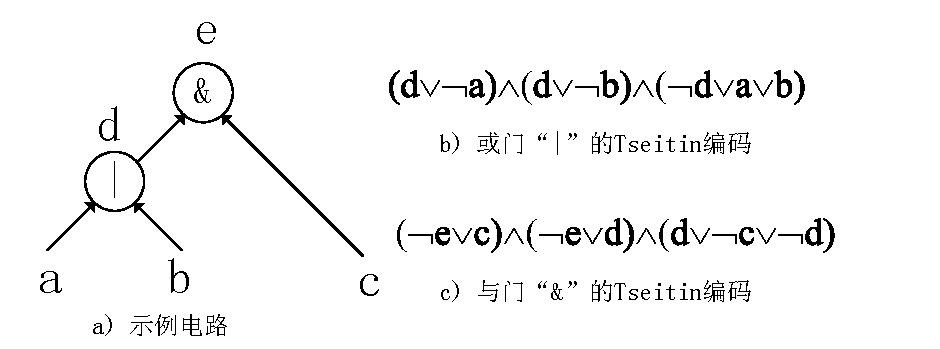
\includegraphics[width=0.8\textwidth]{fig_basic_circuit}
  \caption{示例电路及其编码}
  \label{basic_circuit}
\end{figure}


最简单的SAT求解算法是简单地遍历所有可能的变量赋值,形成树形的二叉搜索空间。对于图\ref{basic_circuit}b)的SAT公式,将导致图\ref{basic_search}所示的二叉搜索树。其中打钩的叶节点表示合法的求解结果。每次对特定变量进行二叉分解的步骤称为决策,每次决策产生一个新的决策层。图\ref{basic_search}的决策层1、2和3分别对应于分别对变量a、b和c进行二叉分解。

\begin{figure}[b] % use float package if you want it here
  \centering
  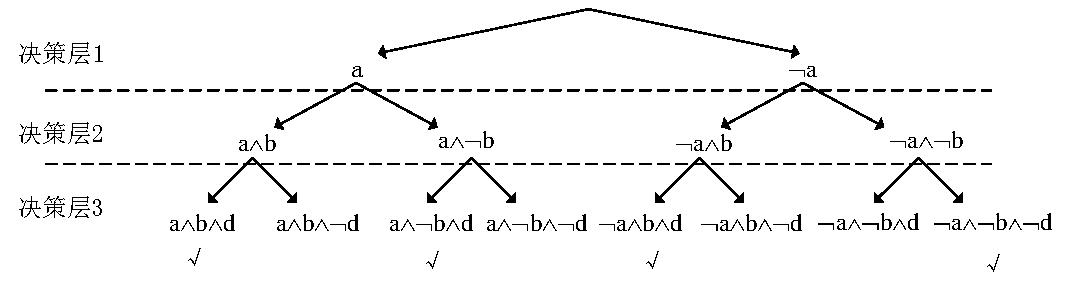
\includegraphics[width=0.8\textwidth]{fig_basic_search}
  \caption{基于完全二叉树遍历的SAT求解}
  \label{basic_search}
\end{figure}

\subsubsection{布尔约束传播(BCP)}
为了使一个特定的SAT公式成立,必须使其中每个子句都成立。
而为了使某个特定子句成立,其中必须存在至少一个文字成立。
因此当在某个子句中,只有一个特定的文字$w$尚未取值,而其他所有文字均取值为$0$时,
则该文字必须取值为$1$。
如果该文字为某个特定变量$v$,这将导致$v$取值为$1$,否则取值为$0$。
这一推导过程称为布尔约束传播。

以图\ref{basic_circuit}b)的或门的Tseitin编码为例,
为了使该公式成立,每个子句都必须成立。
以第一个子句$d \wedge a$为例,当$a$ 为$1$时,
$d \wedge a$化简为$d$,
为了使其成立,$d$必须取值为1。
此时搜索树如图\ref{BCP} 所示。
其中粗线代表在特定决策层内部的BCP 操作。

\begin{figure}[t] % use float package if you want it here
  \centering
  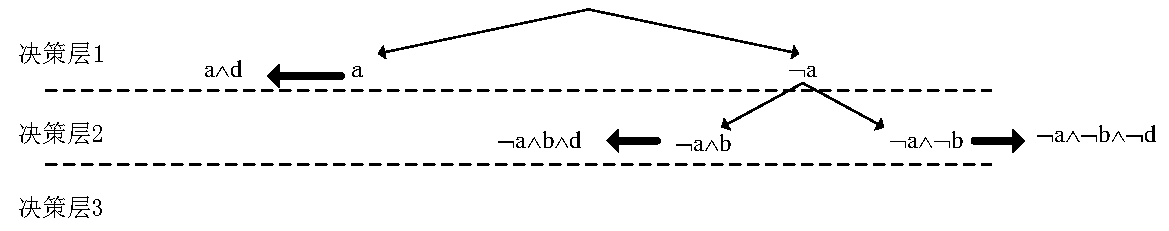
\includegraphics[width=0.8\textwidth]{布尔约束传播}
  \caption{布尔约束传播}
  \label{BCP}
\end{figure}

\subsubsection{冲突指导的子句学习}
冲突指导的子句学习和非正交回溯\upcite{DBLP:conf/iccad/ZhangM02} 是提升SAT求解器性能的另一个重要手段。其中非正交回溯与与本文重点关注的数据结构关系不大,因此将仅描述冲突指导的子句学习。

为了简明起见,仍然使用一个例子描述冲突指导的子句学习。如图\ref{confict}所示的一个二叉搜索树,当到达红色的标记为conflict 的节点时,有$\{a \equiv 0,b \equiv 0, c \equiv 0,d \equiv1,e \equiv 0,f \equiv1\}$。这将导致某个短句中的所有文字均成为0,称这种情况为一个冲突(conflict)。 此时冲突分析算法将对该子句中的每一个文字,沿着如图\ref{confict}粗线所示的BCP 关系逆向回溯,以便找到导致此次冲突的根本原因。假设找到的三个变量分别为$\{c \equiv 0,d \equiv 1,f \equiv 1\}$,这意味着a、b和e与本次冲突无关。无论以后a、b 和e 取任何值,只要遇到$\{c \equiv 0,d \equiv 1,f \equiv 1\}$ 的情况,都不必继续搜索。这意味图\ref{confict}中绿色所示的分支都可以被剪掉。

为了达到这种剪枝效果,将对冲突分析的结果中每个变量取反,以构造一个冲突学习子句。即$\{c \equiv 0, d \equiv 1, f \equiv 1\}$ 将会产生一个冲突学习子句$\{c\vee \neg d \vee \neg f\}$,并加入子句数组。以后每次当c、d和f三个变量中的两个满足$\{c \equiv 0, d \equiv 1, f \equiv 1\}$,则将立即通过冲突学习子句产生一次BCP,使得第三个变量无法满足$\{c \equiv 0,d \equiv 1,f \equiv 1\}$。 这就构成了一次剪枝操作。

\begin{figure}[t] % use float package if you want it here
  \centering
  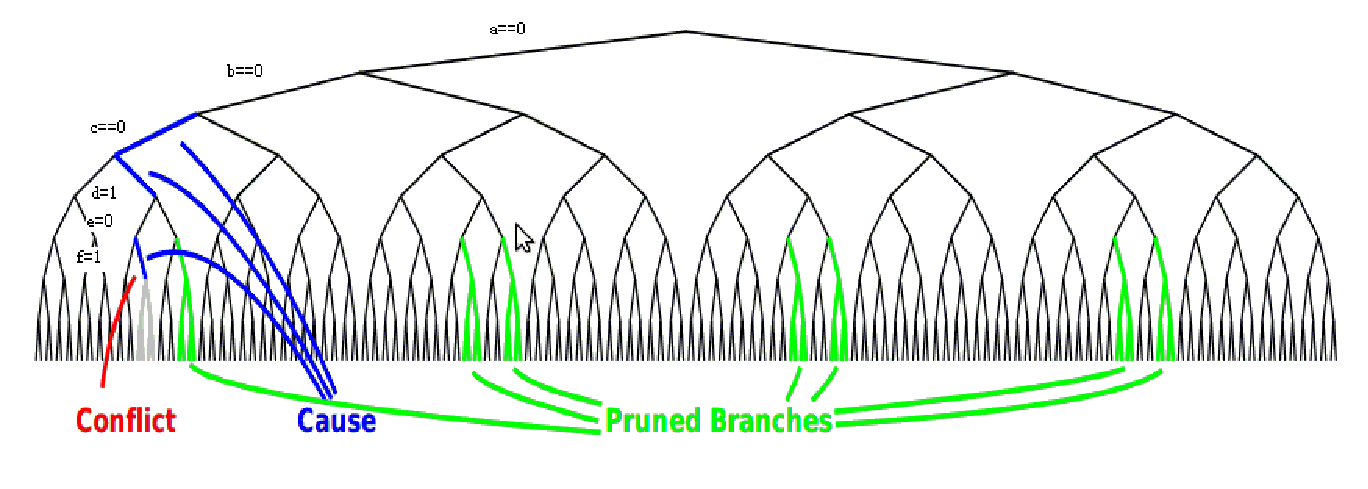
\includegraphics[width=0.8\textwidth]{fig_conflict}
  \caption{冲突指导的子句学习}
  \label{confict}
\end{figure}


\subsubsection{MiniSat 求解器的递增求解机制}\label{subsec_incsat}

本文中,
我们使用MiniSat 求解器\upcite{EXTSAT} 求解所有CNF公式。
和其他基于冲突学习机制\upcite{CONFLICTLEARN}的SAT求解器类似,
MiniSat 从在搜索中遇到的冲突中产生学习短句,
并记录他们以避免类似的冲突再次出现。
该机制能够极大的提升SAT求解器的性能。

在许多应用中,
经常存在一系列紧密关联的CNF公式。
如果在一个CNF公式求解过程中得到的学习短句能够被其他CNF公式共享,
则所有CNF公式的求解速度都能够得到极大的提升。

MiniSat 提供了一个增量求解机制以共享这些学习短句。
该机制包括两个接口函数:
\begin{enumerate}
\item
$addClause(F)$ 用于将一个CNF公式$F$ 添加到MiniSat的短句数据库,
以用于下一轮求解。
\item
$solve(A)$ 接收一个文字集合$A$作为假设,
并求解CNF 公式$F\wedge \bigwedge_{a\in A} a$。
其中$F$是在$addClause$中被加入短句数据库的CNF公式。
\end{enumerate}

基于该机制,
可以针对一个相同的CNF公式$F$,
使用不同的文字集合$A$,
来产生并递增地高效求解不同的$F\wedge \bigwedge_{a\in A} a$。


\subsection{可满足赋值遍历}\label{subsec_relallsat}
多数时候,可以满足特定SAT问题的解并不是唯一的,
求出所有可满足解的过程被称为可满足赋值遍历(简称ALLSAT求解)。

ALLSAT求解由基于SAT求解的可满足赋值遍历算法来实现。
直观上看,调用一次SAT求解器可以获得SAT问题的一个解,也就是一个完整的可满足赋值。
将这个完整的可满足赋值中每一个文字取反,构造出阻断(block)子句并加入到待求解的SAT问题公式中,
以引导SAT求解器避开已搜索过的解。
通过多次重复,最终可以获得SAT问题所有的解。

绝大多数可满足赋值遍历算法致力于将由SAT求解得到的一个完整的赋值扩展为一个包含较多赋值的赋值集合,
以便减少调用SAT求解器的次数并压缩存储赋值解的空间开销。
文献\upcite{SATUNBMC}提出了第一个此类算法。
他在SAT求解器求解过程中构造一个蕴含图,
用以记录每个赋值之间的依赖关系。
每个不在该图中的赋值变量都可以从最终结果中剔除。
在文献\upcite{MINASS} 和\upcite{REPARAM}中,
每个变量如果在其不被约束的情况下不能使$obj\equiv 0$ 被满足的话,
则该变量可以从最终结果中剔除。
在文献\upcite{MINCEX} 和\upcite{PRIMECLAUSE,EFFCON}中,
冲突分析方法被用于剔除与可满足性无关的变量。
在文献\upcite{MEMEFFALLSAT}中,
变量集合被划分为重要变量和非重要变量集合。
搜索过程中重要变量的优先级高于非重要变量。
因此重要变量子集构成了一个搜索树,
而该树的每一个叶节点是非重要变量的一个搜索子树。
%Tobias Nopper et al.\upcite{CMPMINCEX} propose an counterexample minimization algorithm for incomplete designs that contain black box.
Cofactoring \upcite{EFFSATUSMCCO} 则通过将非重要变量设置为SAT求解器返回的值以缩减搜索空间。

另一类算法通过Craig插值以扩大解集合。
文献\upcite{InterpBoolFunction}提出了第一个此类算法。
该算法构造两个相互矛盾的公式,并从他们的不可满足证明中抽取Craig 插值。
在文献\upcite{interpNoProof}中,
Craig插值的产生过程类似于传统的可满足赋值遍历算法。
不过其扩展算法包含两步,
分别对应于两个参与计算的公式。
该算法是第一个不需要产生不可满足证明的Craig插值算法。

\subsection{Craig插值的原理和实现}\label{sec_craigimp}
在通常的SAT求解器,
包括本文使用的MiniSat\upcite{EXTSAT}中,
要求待求解的公式被表示为CNF格式。
其中一个公式是多个子句的合取(conjunction),
而每一个子句是多个文字的析取(disjunction),
而每个文字是一个布尔变量$v$或者其反$\neg v$。
如公式$(v_0\vee\neg v_1\vee v_2)\wedge(v_1\vee v_2)\wedge(\neg v_0\vee v_2)$,
包含子句$v_0\vee\neg v_1\vee v_2$,$v_1\vee v_2$和$\neg v_0\vee v_2$。
而子句$v_0\vee\neg v_1\vee v_2$包含文字$v_0$, $\neg v_1$和$v_2$。

当存在一个变量$v$,
使得一个子句$c$中同时包含两个文字$v$和$\neg v$,
则称$c$为tautological的。
我们通常假设有待SAT求解器求解的公式中所有的子句都是非tautological的。

假设公式$F$的布尔变量全集为$V$。
若存在对$V$的赋值函数$A:V\to \{0,1\}$,
使得$F$中的每个子句均能取值为1,
则称$F$是可满足的,
此时SAT求解器能够找到赋值函数$A$。
否则称$F$为不可满足的,
此时SAT求解器能够产生如下一小节所述的不可满足证明。

\subsubsection{不可满足证明}
对于两个子句$c_1=v\vee A$和$c_2=\neg v\vee B$,
当$A\vee B$是tautological时,
$A\vee B$称为它们的\textbf{resolvant}。
而$v$称为它们的\textbf{pivot}。
易知以下事实:

\begin{equation}
\begin{array}{ccc}
&resolvant(c_1,c_2) = \exists v, c_1\wedge c_2 &\\
&c_1\wedge c_2 \to resolvant(c_1,c_2)&
\end{array}
\end{equation}

\begin{definition}
对于不可满足公式$F$,
假设其子句集合为$C$,
则其不可满足证明$\Pi$是一个有向无环图$(V_{\Pi},E_{\Pi})$,
其中$V_{\Pi}$是子句集合,
而$E_{\Pi}$是连接$V_{\Pi}$中子句的有向边集合。
$\Pi$满足如下要求:
\begin{enumerate}
\item 对于节点$c\in V_{\Pi}$:
  \begin{enumerate}
    \item 要么$c\in C$,此时称$c$为$\Pi$的根
    \item 或者$c$有且仅有两个扇入边$c_1\to c$和$c_2\to c$,
    使得$c$是$c_1$和$c_2$的resolvant。
  \end{enumerate}
\item 空子句是$\Pi$的唯一一个叶节点。
\end{enumerate}
\end{definition}

直观的说,
$\Pi$就是一棵树,
以子句集合$C$的子集为根,
以空子句为唯一叶节点。
而每个节点$c$的两个扇入边$c_1\to c$和$c_2\to c$代表了一个resolving关系$c:=resolvant(c_1,c_2)$。

包括本文使用的MiniSat求解器\upcite{EXTSAT}在内的许多SAT求解器,
当公式不可满足时都将产生一个不可满足证明$\Pi$。

\subsubsection{Craig插值算法}

根据文献\upcite{Craig},
给定两个布尔逻辑公式$A$ 和$B$,
若$A\wedge B$ 不可满足,
则存在仅使用了$A$ 和$B$共同变量的公式$I$ ,
使得$A\Rightarrow I$且
$I\wedge B$不可满足。
$I$ 被称为$A$针对$B$的Craig插值\upcite{Craig}。

目前最常见且最高效的产生Craig插值的算法是
McMillan算法\upcite{interp_McMillan} 。
其基本原理描述如下。

对于上述公式$A$和$B$,
已知$A\wedge B$不可满足,
而$\Pi$是SAT求解器给出的不可满足证明。
当一个变量$v$同时出现在$A$和$B$中时,
我们称其为全局变量。
若$v$只出现在$A$中,
则称其为$A$本地变量。

对于文字$v$或者$\neg v$,
当变量$v$是全局变量或者$A$本地变量时,
称该文字为全局文字或者$A$本地文字。

对于子句$c$,
令$g(c)$为$c$中所有全局文字的析取,
而$l(c)$为$c$中所有$A$本地文字的析取。

例如,
假设有两个子句$c_1=(a\vee b\vee\neg c)$ 和
$c_2=(b\vee c\vee\neg d)$。
并假设$A=\{c_1\}$和$B=\{c_2\}$。
则$g(c_1)=(b\vee\neg c)$,
$l(c_1)=(a)$,
$g(c_2)=(b\vee c)$,
$l(c_2)=FALSE$。


\begin{definition}\label{def_gencraig}
令$(A,B)$为一对公式,
而$\Pi$是$A\wedge B$的不可满足证明,
且其唯一叶节点是空子句$FALSE$。
对于每一个节点$c\in V_{\Pi}$,
令$p(c)$为如下定义的一个公式:
\begin{enumerate}
\item 如果$c$是根节点则
  \begin{enumerate}
    \item 如果$c\in A$则$p(c)=g(c)$
    \item 否则$p(c)=TRUE$
  \end{enumerate}
\item 否则令$c_1$和$c_2$分别是$c$的两个扇入节点,而$v$是他们的pivot变量
  \begin{enumerate}
    \item 如果$v$是$A$本地变量,则$p(c)=p(c_1)\vee p(c_2)$。
    \item 否则$p(c)=p(c_1)\wedge p(c_2)$。
  \end{enumerate}
\end{enumerate}
\end{definition}

上述定义\ref{def_gencraig}是构造性的,
已经给出了从不可满足证明$\Pi$得到最终的Craig插值的算法,
即以$\Pi$的根节点为起点,
为每一个$c$计算相应的$p(c)$,
直至到达最终的唯一叶节点$FALSE$。
我们有以下定理:

\begin{theorem}
定义\ref{def_gencraig}为唯一叶节点$FALSE$产生的$p(FALSE)$即为
$A$相对于$B$的Craig插值。
\end{theorem}

该定理的详细证明可见文献\upcite{DBLP:journals/tcs/McMillan05}。

计算$A$相对于$B$的Craig插值的时间复杂性为$O(N+L)$,
其中$N$是$\Pi$中包含的节点个数$|V_{\Pi}|$,
而$L$是$\Pi$中的文字个数$\Sigma _{c\in V_{\Pi}}|c|$。
而所产生的插值可以视为一个电路,
其空间复杂性为$|O(N+L)|$。
当然,
$\Pi$的尺寸在最坏情况下也是$A\wedge B$的尺寸的指数。

%\subsection{对偶综合}\label{subsec_relallsat}


\section{面向软硬件设计验证的可满足问题求解}
可满足问题(SAT)\upcite{SATtheory}是硬件电路设计和软件可信验证领域\upcite{HardwareSAT,softwareSAT} 共同关注的重要问题。许多重要的电路设计和软件验证问题均可转换为可满足性问题,并由SAT求解器求解。随着集成电路制造工艺的发展,在单个芯片内集成的晶体管个数将在2020年接近一千亿;而社会信息化程度的提高促使软件系统越来越复杂,以Linux操作系统为例,在2008 年仅其内核代码就已经突破1千万行。软硬件系统的规模日益增大,服务于硬件设计和软件验证的SAT求解器的运算量也急剧攀升。在过去的10年,作为形式化工具基本引擎的SAT 求解器性能已经显著提升,几分钟内即可处理数百万变量和数亿子句,但是依然无法满足日益增长的计算要求。

传统的硬件辅助与设计(EDA)综合与验证工具的核心框架通常包含以下主要功能模块:

1.抽象问题表示:该模块用于管理与特定推理过程和引擎无关,但是与问题本身密切相关的数据结构,如简化布尔电路(Reduced Boolean circuits)\upcite{DBLP:conf/tacas/AbdullaBE00}和
与非图(And-Inverter Graph)\upcite{Brummayer06localtwo-level}等。

2.问题编码:该模块用于将特定的抽象问题表示,转换为满足特定推理引擎,
如二叉决策图(简称BDD)\upcite{DBLP:journals/tc/Bryant86} 或SAT要求的数据结构,以便进行高效的推理工作。针对SAT推理引擎,该模块通常使用在空间和时间方面均具有多项式复杂性的Tseitin\upcite{Tseitin} 编码。

3.BDD和SAT推理引擎:这两个模块负责具体的推理工作。
绝大多数EDA工具和软件验证工具的核心推理引擎为二叉决策图(BDD)和可满足求解器(SAT)。其中BDD受到归一化表示方式导致的状态空间爆炸问题的困扰,通常仅用于需要归一化特性的小规模推理问题,如抽象谓词的表示等。而SAT则通常较少受到状态空间爆炸的影响,且天生具有内在的并行性和可扩展性;另一方面SAT问题是NP难问题,其求解时间和问题结构相关,对计算资源的需求也随具体问题而不同。

软件程序验证工具也具有类似于硬件设计验证工具的核心框架。
SAT求解器通常是作为核心推理引擎集成到具体问题求解器中。
因此,从逻辑流程上看,
硬件和软件形式化验证通常都是通过抽象问题表示之后再进行问题编码,
而后将问题的可满足性求解过程交给SAT 求解器完成,
流程如图\ref{verfication-procedure}所示。

\begin{figure}[t] % use float package if you want it here
  \centering
  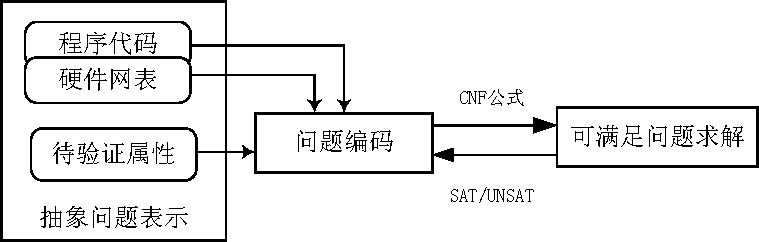
\includegraphics[width=0.8\textwidth]{验证流程}
  \caption{基于SAT求解的软硬件验证流程}
  \label{verfication-procedure}
\end{figure}

因此将软硬件设计验证中产生的复杂SAT 问题外包到云或网格环境下,利用其提供的弹性计算资源,成为一种有吸引的解决方案。
科研机构和商业公司也已经开展了在云和网格环境下进行SAT问题求解的研究
\upcite{DBLP:conf/IEEEcloud/BrunM12,Nordugrid,DBLP:journals/concurrency/ChrabakhW07,OneSpin,CloudSMT}。
如美国华盛顿大学研究小组推出支持云SAT求解的sTile系统\upcite{DBLP:conf/IEEEcloud/BrunM12};
芬兰阿尔托大学研究小组推出基于NorduGrid的SAT求解器\upcite{Nordugrid};
美国圣巴巴拉大学研究小组推出GridSAT系统\upcite{DBLP:journals/concurrency/ChrabakhW07};
形式化验证服务提供商OneSpin 公司和Plunify公司于2013年,
联合推出了面向云平台的基于SAT求解的硬件验证商业服务\upcite{OneSpin}。

\section{开放环境下数据隐私的安全威胁}
云计算和网格依托于互联网,与互联网这种开放环境的便利快捷相伴而生的是,安全威胁也无处不在。
一方面,公有云和网格计算节点均直接部署在广域网上,与用户处于不同的安全域。
用户的服务请求可能面临来自网络中的多重威胁;
另一方面,云服务提供商或是网格计算节点无法证明其内部行为可以信任。

由于网格计算是由松散耦合的高端计算设施组成\upcite{Nordugrid},网格环境下恶意计算节点是客观存在的\upcite{HV-grid};
而在云计算环境下,虽然云硬件平台提供商及其基础设施(虚拟层)是可被信赖,在其上运行的虚拟机却不总是可以信赖的。
文献\upcite{AMI}指出,著名的云计算提供商亚马逊的EC2受到了虚拟机影像滥用的困扰,被污染虚拟机映像会迅速扩散到整个社区;
而文献\upcite{InformationLeakageofCloud} 则指出了处于同一台物理机器上的虚拟机之间攻击的可能性。
与此相照应,早在2007年,
《华盛顿邮报》就披露了客户关系管理领域著名的云服务提供商Saleforce.com由于受到安全攻击而导致大量租户数据泄露与丢失\upcite{washingtonPostSaleForce};
2010 年下半年谷歌解雇了两名入侵租户的私有账户以获取隐私数据的员工\upcite{googelFiresTwoEmployees}。
Gartner 公司发布的研究报告\upcite{gartner70}显示,所采访的企业中70\%以上认为出于对数据安全性与隐私保护的怀疑,
在近期内不会采用云计算技术。
RSA 首席技术官也指出\upcite{rsaSafe},在企业将现有的应用向第三方云服务提供商提供的云环境迁移过程中,
要考虑的首要问题是对云计算的数据安全问题。
此处的安全不仅指数据的可用,更加注重的是数据的隐私保护。
针对OneSpin公司推出的硬件形式化验证云服务,新闻评论\upcite{oneSpinsafe}指出验证数据的隐私是用户最为关心的因素。

而针对计算结果的安全性,对早期的志愿计算SETI@home项目的统计发现\upcite{HV-grid},这类基于网格的开放计算环境存在三类威胁:
\textbf{私心的计算参与者}:由于计算结果具有稀缺性,私心的计算参与者会出现奇货可居的意识,他们会完全遵照协议的规定,尽力计算出正确结果,但会出于利益原因,将有价值的结果信息透露给第三方,从而损害用户的隐私安全。
\textbf{懒惰的计算参与者}:由于大计算量会耗费很多计算资源,出于节约计算成本的考虑,计算参与者可能不按照约定来进行足量的计算,以此来节省开销,使用部分结果来作为最终结果。
\textbf{恶意的计算参与者}:可能出于某种目的,计算参与者完全违反协议规定,随意返回错误结果来欺骗用户,误导用户决策。
而在2009年对云计算模型和网格计算模型的比较一文\upcite{DBLP:journals/corr/abs-0901-0131} 中,Ian Foster 指出云计算在安全措施设计成熟度还远不及网格,这就使得网格计算下影响结果正确性的威胁也很可能对云计算环境造成影响。

这些事实指出,外包到云计算或网格这类开放环境下的SAT问题,
由于计算模式将数据和处理的控制权从用户转移至云服务方,导致具体的处理过程用户不可控;
其输入和输出数据可能会被未授权的第三方访问,
这些潜在的威胁者可能会从这些数据中获取有价值的信息。
糟糕的是,即使发生了上述信息泄露的情况,如果不辅助以技术手段,用户难以察觉和追踪;
更为恶劣的情况是,部署在网格或云环境下的SAT求解器可能会被迫使返回错误的结果。

来源于软硬件验证的SAT问题,可能遭受硬件结构信息泄露的问题;Roy\upcite{csRoy} 和Fu\upcite{csFu}的工作指出了从CNF 公式中抽取电路结构信息的可能性。Zvika\upcite{OBfuscationd-CNFs}、Yuriy Brun\upcite{DBLP:conf/IEEEcloud/BrunM12} 等人的工作也指出在云计算环境下进行SAT问题求解需要解决隐私保护问题。另一方面,Du\upcite{HV-grid} 将某些复杂SAT问题的解称作高价值稀有事件,指出SAT问题的解也应该被视作为隐私;如来源于密码破解的SAT问题,奇货可居的计算参与者可能会因利益问题而将其泄露给第三方。

\section{开放计算环境下可满足问题求解的隐私保护问题}
开放环境下的这些威胁将SAT计算服务的潜在用户置于进退维谷的境地:
使用公共的云计算或网格计算基础设施在系统维护性和可用性上面具有较高的性价比,
但却会面临隐私泄露和错误结果等安全问题的困扰。
在开放计算环境下,计算数据的隐私保护问题看起来是一个不可能完成的问题:由于计算是在开放环境下完成的,未经加密处理的原始输入和输出数据势必会引发泄露的风险,而经过传统加密算法处理之后的计算数据由于对计算不再透明,因而丧失了可计算性。因此在保持可计算性的前提下,讨论SAT数据的隐私保护,成为了开放计算环境下的最大挑战。

2009 年,Gentry 等人针对开放计算环境下的数据隐私保护问题,提出完全同态加密的概念。
这一概念描绘了开放环境下计算外包的美好愿景:经过完全同态加密,在保持数据隐私性的同时,仍然可保持原有数据的可计算性。完全同态加密的理论基础是,由于任何计算都可以分解为一系列微观加乘计算,并且在有限步内对加乘计算透明的加密算法确实存在。
因而任意的计算都可以分解为一系列的有限次针对加密数据的加乘计算。
这无疑从理论上扫清了开放环境下计算外包的安全障碍。但是,由于完全同态加密需要将计算分解为细粒度的有限步加乘计算。
所带来的昂贵计算开销,使其距离实用化还有相当的距离。

同样为了解决外包计算的数据隐私保护,Atallah等提出了针对具体问题,进行计算数据伪装的概念。例如针对矩阵求解类计算,将有待外包的数据与随机对角矩阵进行矩阵乘,对外包的矩阵数据进行伪装加密。
由于矩阵计算的可逆性,伪装加密后结果可以通过可逆的矩阵运算得到。数据伪装方法充分利用了问题的特点,不改变原有计算过程和数据的外在形式,是一种直接实用的方案。但目前针对SAT 问题的数据伪装的研究还处于空白。

作为一种基础的计算引擎,软硬件设计问题中的SAT问题具有其内在的特点:任何硬件设计和软件程序都可以表示为与或非等门的集合。
本文从实用化的角度出发,希望在复用原有求解器的前提下,探讨软硬件设计、验证领域中SAT 问题的隐私保护方法。

\subsection{CNF公式中的结构信息}\label{CNF structure}
%\textbf{Circuit structure in CNF formula}\label{CNF structure}
%Since we want to protect circuit structure in CNF formula,
%let's first study how the circuit can be recovered from CNF formula.
%Literatures\upcite{csRoy,csFu} have proposed algorithms to recover circuit structure from CNF formula in details.
%Before discussing them, some concepts should be introduced first.
CNF公式是SAT求解的输入数据,来源于软硬件验证及设计中的CNF公式中会包含硬件电路结构信息;
文献\upcite{csRoy,csFu}给出了从CNF公式中获取电路结构信息的算法细节,首先了解算法中用到的概念。
%
%\begin{definition}[CNF signature]
%CNF signature of gate $g$ is its Tseitin encoding $Tseitin(g)$.
%Each clause in CNF signature is called characteristic clause.
%A characteristic clause containing all variables in CNF signature is a \textbf{key clause}.
%Variable corresponding to output of a gate is called \textbf{output variable}.
%\end{definition}
\begin{definition}[CNF标记]
门$g$的CNF标记就是它的Tseitin编码$Tseitin(g)$。
CNF标记中的每个子句称为门的\textbf{特征子句}。
包含门中所有变量的特征子句称为\textbf{关键子句}。
对应于门输出的变量称为\textbf{输出变量}。
\end{definition}

公式(\ref{eqn_andinv})中的 AND2门,
$\neg e\vee c$ 是它的一个特征子句,
$e\vee \neg c\vee\neg d$是它的关键子句。
$e$是输出变量。

文献\upcite{csRoy}指出,
在一种编码规则下,具有相同特征函数的门必然会被编码成为相同的CNF 标记,也就是相同的子句集合。
通过探索这种结构特征可以恢复电路结构,已知的结构检测算法基于以下定义的有向超图和二分图概念。

\begin{definition}[超图]\label{Hypergraph}
 以CNF公式中的子句为节点、变量为边,形成的图称为超图(Hypergraph)。
 超图$G(V,E)$ 中:
 $V$中每个节点对应$F$中一个子句;
 $E$中每条边对应$F$中一个变量。
 如果两个子句包含相同的变量,就在两个子句之间连接一条边,并用变量标注。
\end{definition}

在超图表示方式下,存在具有不同CNF标记的两个门,却具有相同超图表示的情况,
如AND3和OR3,均对应图\ref{graph}a)中的超图。
为了克服该问题,在电路结构检测算法\upcite{csRoy}中,使用有向超图进行区分。

\begin{definition}[有向超图]
在定义\ref{Hypergraph}给出的超图基础上,
根据子句中文字的正负、为边添加标记,
形成的图称为有向超图(Directed Hypergraph)。
\end{definition}

\begin{definition}[二分图]
将子句和变量均视为节点,同时将变量和子句的从属关系视为边,形成的图称为二分图(Bipartite Graph)。
在二分图$G(V,E)$中:
$V$中每个顶点对应于集合中的一个子句或一个变量,即$V=V_{cls}\bigcap V_{var}$,其中$V_{cls}$为子句集合、$V_{var}$ 为变量集合。
$E$中的每条边对应于一个子句/变量对,
如果变量出现在子句中,就在变量和子句之间连接一条边;变量为负值则对应一条负边,反之为正边。
\end{definition}

以AND门为例,AND3门的超图如图\ref{graph}a)所示;
其有向超图对应于图\ref{graph}b),其中使用$\uparrow$表示正,┼ 表示负;
其二分图对应于图\ref{graph}c) 所示的二分图。
\begin{figure}[t]
  \centering
  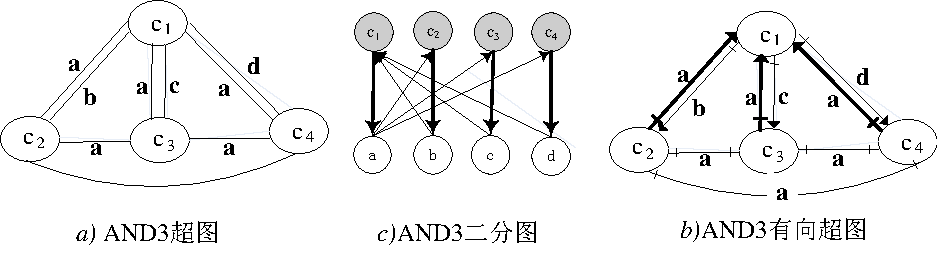
\includegraphics[width=0.8\textwidth]{超图二分图}
  \caption{超图和二分图}
  \label{graph}
\end{figure}

基于上述定义,CNF公式可以表示为包含多种CNF特征子图的超图或二分图。
这种图结构使得利用基于子图同构和模式匹配技术来恢复出电路结构和程序结构信息成为可能。

\subsection{SAT问题隐私保护的对象}
基于上述概念,
CNF公式可以转化超图$G$,
在图中匹配常用的CNF标记,通过同构子图的方式即可恢复出CNF公式携带的门信息。
进一步,可用最大无关集来表示恢复出来的电路信息。
基于关键子句和CNF标记的模式匹配还可以检测出所有门,并构建最大匹配门的子集。
除了门的结构信息,在来源于软硬件验证的CNF公式还包含了状态迁移关系。
Roy\upcite{csRoy}和Fu\upcite{csFu} 给出了具体的实现技术。
潜在的攻击者可以利用这些技术手段恢复出电路结构,并得到电路的状态迁移关系。
因此,CNF标记和关键子句是特别需要保护的重要信息。

另一方面,在验证领域,某些SAT问题的解反映了该系统的某些特性是否达到,因此解也应作为隐私加以保护。

\section{本文的主要工作}
来源于软硬件验证和设计的SAT 问题,
由于其CNF公式和其解中包含了电路结构以及电路迁移关系等敏感信息,在开放计算环境下求解,必须防止这些敏感信息的泄露。
本文的工作也围绕着保护上述敏感信息展开。

\subsection{已有工作的局限}
针对开放计算环境下的计算数据隐私保护问题,2009年Gentry\upcite{DBLP:conf/stoc/Gentry09} 等人开创性提出完全同态加密的概念。
经过完全同态加密,在保持数据隐私性的同时,仍然可保持原有数据的可计算性。由于任何的计算都可以分解为一系列微观加乘计算,因此寻找可保持对加乘的加密算法成为了一个努力的方向。
但是由于计算需要被分解为细粒度的有限步的加乘操作,因此同态加密后的计算效率一直制约着该方法的实用化。

针对CNF公式隐私保护方面相关的研究才刚刚开始,2013年Brakerski\upcite{OBfuscationd-CNFs} 等人面向云计算环境,首次探讨了使用多线性映射和坡度编码策略对d-CNF进行混淆的方法。
使用随机和带有噪声的编码,并提供测试过程来确保编码元素的等价。
这种方法基于有限加速假设,混淆后的CNF使用最原始的二叉树搜索的方法进行求解,无法利用目前经典的SAT求解器。

Yuriy Brun\upcite{DBLP:conf/IEEEcloud/BrunM12} 等人则使用了stile数据分布的模式,通过将数据条块计算,提高攻击者获得完整CNF 公式难度,以此降低数据被窃取的可能性。
该方法目前也仅仅支持简单的二叉遍历赋值求解方法,无法利用已有的SAT 求解加速算法。

上述的工作都试图重新构造求解器,无法利用目前已有的求解器研究成果。

\subsection{研究内容与创新点}
鉴于目前的研究现状,本文力图从SAT问题特性出发,寻求具有实用性的隐私保护方法。图\ref{fig:103}给出了本文的主要研究内容。

\begin{figure}[t] % use float package if you want it here
  \centering
  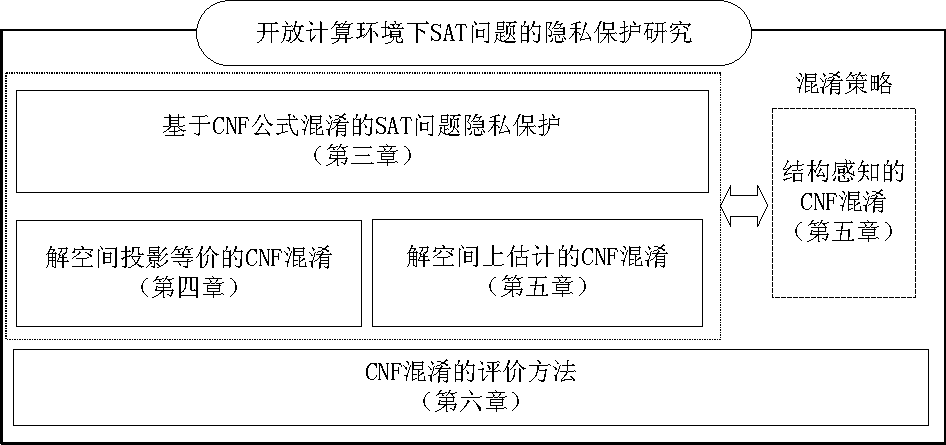
\includegraphics[width=0.8\textwidth]{fig103}
  \caption{本文研究内容}
  \label{fig:103}
\end{figure}

本文受国家高技术研究和发展计划“智能云服务与管理平台核心软件及系统”(项目编号2013AA01A212)和国家自然科学基金项目“面向通讯应用的自动对偶综合研究”(项目编号61070132)的支持,主要贡献和创新点如下:

1. 开放环境下基于加噪CNF混淆的SAT求解框架。
CNF公式混淆是保证开放环境下的SAT求解隐私性的重要手段。现有的方法基于双射或多射群加密,通过分段坡度编码对CNF 公式进行混淆,从而隐藏CNF公式中携带的结构信息。
但是这种方法改变了原有CNF公式的外部表示,需要设计新的求解算法。
并且在目前仅可使用全空间遍历的方法进行求解,无法利用已有成熟的SAT 求解算法,因此极大降低了其实用性。
本文通过对CNF公式自身逻辑特点的分析,提出了基于加噪思路的混淆算法。通过在原始CNF公式中无缝的混入噪音公式,在隐藏原有的结构信息的同时,保持原有的CNF 数据形式和解空间,从而复用目前已有的求解算法。
这就在算法的实用性和隐私保护上取得了良好的折中。
本文从理论上证明了算法的正确性并通过大量的仿真实验验证了算法的性能。

2. 解空间上估计的CNF混淆算法。
由于SAT求解时,输出数据也包含了敏感信息。
在研究了隐藏结构信息的CNF混淆算法之后,本文进一步研究了隐藏CNF 解的混淆方法。针对输出信息保护,本文提出了解空间上估计的CNF混淆算法。
通过扩展噪音公式解空间,使得混淆后SAT问题的解空间为原始解空间的上估计。
通过引入噪音解实现对原始解的隐藏。
本文从理论上充分证明了算法的正确性,并通过大量的仿真实验验证了方法的有效性和性能。

3. 混淆后公式的求解效率是在混淆算法有效性的一个特别重要的指标,也是基于加噪的混淆算法区别于其他混淆算法的一个重要因素。
由于加噪的过程改变了公式的内在结构,并且SAT问题自身特点,使得其问题复杂度会随着结构的变化出现跃变。
针对这一情况,本文针对硬件验证中常用的CNF结构进行分析,提出了跃变敏感的混淆策略,使得混淆后的CNF公式求解难度不会大于原始公式求解难度。
特别针对对偶综合这一SAT问题的实例算法进行了分析。从理论上验证了算法的可用性。

4. CNF混淆算法的有效性评价。
混淆算法保证混淆后的CNF公式可用已有的求解器求解,并且可以用较小的开销恢复出原始的解。
但是除此之外,在开放环境下为保证SAT 计算外包的顺利实施,混淆算法仍然需要满足其他的特性。
结合程序混淆的有效性评价标准,本文抽象出CNF公式混淆的有效性评价标准。
通过对混淆策略的细分,针对两种混淆策略进行定量分析和定性评价,为设计出更好的混淆策略提供了依据。

上述各部分研究内容之间的关系参见图1.3。
\section{论文组织结构}
论文共分六章,组织结构如下:
%TO DO 论文共分七章,组织结构如下:

第一章为绪论,介绍SAT求解的基本概念、特点、应用以及安全可验证计算的研究现状。分析CNF公式混淆算法的研究意义和挑战,并简述本文的研究内容和组织结构;

第二章为相关研究,对科学计算外包隐私保护、安全可验证计算以及程序混淆等相关概念进行了系统和全面的介绍,分析了现有工作的特点和适用性;

第三章研究SAT问题求解中输入数据的隐私保护问题,从实用性的角度出发,提出了基于加噪的CNF混淆算法。
在保证求解算法和解空间不变的前提下,通过混入噪音变量和子句来实现CNF公式内部结构信息的隐藏;

第四章在前述开创性工作的基础上,针对高危险外包计算环境,针对可能出现的ALLSAT攻击,通过引入具有簇形解的噪声CNF 公式,进一步提高混淆算法的鲁棒性;

第五章研究SAT问题求解中输出数据的隐私保护问题,提出了解空间上估计的CNF混淆方法,通过混入用户可剔除的噪声解来隐藏真实的解信息;
另一方面,研究SAT问题求解中输入数据中结构信息的增强型隐藏方法,提出在感知原有公式结构的基础之上,加入可构成合法结构的噪声变量和子句,来实现CNF公式内部结构的保真隐藏,以提高应对基于模式识别和同构检测等隐私攻击的防范能力;

%%第六章研究相变敏感的混淆算法,希望对混淆后的CNF公式求解效率进行有效控制。
第六章研究SAT问题混淆算法的有效性评价问题,希望通过对有效性标准的提取,为设计更为有效的混淆算法提供指导。
%
%第七章总结全文并展望未来的工作。

第七章总结全文并展望未来的工作。
最后是致谢、博士期间撰写的论文、参加的科研工作以及参考文献。

% !Mode:: "Tex:UTF-8"
\chapter{基于余因子和Craig插值的迭代特征化算法}
\label{chap:2}



\section{问题描述}

在形式化验证和综合领域,
对于两个存在某种内在联系的逻辑向量$\vec{a}$和$\vec{b}$,
有两种不同的方式表达他们之间的联系:关系和函数。

其中,
关系$R(\vec{a},\vec{b})$更具一般性,
能够表达$\vec{a}$和$\vec{b}$之间的任意对应。
尤其是一对多的对应,
这是关系比函数具有更强描述能力的地方。
这种一般性在形式化验证中广泛用于描述非确定性行为以扩展描述能力,
以及构造抽象模型\upcite{DBLP:conf/cav/ClarkeGJLV00}以削减计算复杂性等。

而另一方面,
函数是关系的一种受限形式。
如果$R(\vec{a},\vec{b})$满足以下要求,
则能将其转换为相应的函数$\vec{b}:=f(\vec{a})$:
对$\vec{a}$的任意取值$x\in[\![\vec{a}]\!]$,
均存在且仅存在唯一的$y\in[\![\vec{b}]\!]$,
使得$R(\vec{a},\vec{b})$。
在实际的软硬件设计与验证领域,
存在大量的情况需要从一个关系中获得相应的函数。
如在自动激励生成算法中从约束描述产生相应的激励函数\upcite{DBLP:conf/dac/YuanAAP03},
证明导引抽象中的抽象模型构造\upcite{DBLP:conf/fmcad/AmlaM04},
以及本文中推导控制流谓词和特征化解码器等。

以图\ref{fig_relation}为例。
对于图\ref{fig_relation}a)中的一对一映射,
我们可以使用布尔函数$y_1=x_1\wedge x_2$和$y_2=\neg x_1\wedge \neg x_2$表示。
而另一方面,
对于图\ref{fig_relation}b)中的布尔关系,
并不存在相应的布尔函数,
因为$(x_1,x_2)=(0,1)$的情形被映射到了多个$(y_1,y_2)$的组合。
而这种情况可以使用布尔关系$R=(\neg x_1\wedge\neg x_2\wedge \neg y_1\wedge y_2)
\vee(\neg x_1\wedge x_2\wedge \neg y_1\wedge \neg y_2)
\vee(\neg x_1\wedge x_2\wedge y_1\wedge y_2)
\vee(x_1\wedge \neg x_2\wedge \neg y_1 \wedge \neg y_2)
\vee(x_1\wedge x_2\wedge y_1\wedge \neg y_2)$。

\begin{figure}[t]
\begin{center}
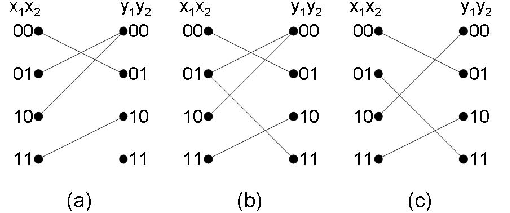
\includegraphics[width=\textwidth]{relation}
\end{center}
\caption{关系和函数的布尔映射}
  \label{fig_relation}
\end{figure}



在本章中,
我们首先在小节\ref{sec_craigimp}描述Craig插值的基本原理,
然后在小节\ref{sec_iterativecraig}中将其扩展到包含额外变量$\vec{c}$ 的更一般情形$R(\vec{a},\vec{b},\vec{c})$。

\section{Craig插值的原理和实现}\label{sec_craigimp}
注意本小节描述的Craig插值基本原理不是我们的原创,
而是为了方便上下文的叙述从\upcite{DBLP:conf/cav/McMillan03} 移植至此。
\subsection{相关背景知识和记法}
在通常的SAT求解器,
包括本文使用的MiniSat\upcite{EXTSAT}中,
要求待求解的公式被表示为CNF格式。
其中一个公式是多个短句的合取(conjunction),
而每一个短句是多个文字的析取(disjunction),
而每个文字是一个布尔变量$v$或者其反$\neg v$。
如公式$(v_0\vee\neg v_1\vee v_2)\wedge(v_1\vee v_2)\wedge(\neg v_0\vee v_2)$,
包含短句$v_0\vee\neg v_1\vee v_2$,$v_1\vee v_2$和$\neg v_0\vee v_2$。
而短句$v_0\vee\neg v_1\vee v_2$包含文字$v_0$, $\neg v_1$和$v_2$。

当存在一个变量$v$,
使得一个短句$c$中同时包含两个文字$v$和$\neg v$,
则称$c$为tautological的。
我们通常假设有待SAT求解器求解的公式中所有的短句都是非tautological的。

当存在一个假设公式$F$的布尔变量全集为$V$。
若存在对$V$的赋值函数$A:V\to \{0,1\}$,
使得$F$中的每个短句均能取值为1,
则称$F$是可满足的,
且SAT求解器能够找到赋值函数$A$。
否则称$F$为不可满足的。

\subsection{不可满足证明}
对于两个短句$c_1=v\vee B$和$c_2=\neg v\vee C$,
当$A\vee B$是非tautological的时,
$A\vee B$称为他们的resolvant。
而$v$称为他们的pivot。
易知以下事实:

\begin{equation}
\begin{array}{ccc}
&resolvant(c_1,c_2) = \exists v, c_1\wedge c_2 &\\
&c_1\wedge c_2 \to resolvant(c_1,c_2)&
\end{array}
\end{equation}

\begin{definition}
对于不可满足公式$F$,
假设其短句集合为$C$,
则其不可满足证明$\Pi$是一个有向无环图$(V_{\Pi},E_{\Pi})$,
其中$V_{\Pi}$是短句集合,
满足如下要求:
\begin{enumerate}
\item 对于节点$c\in V_{\Pi}$:
  \begin{enumerate}
    \item 要么$c\in C$,此时称$c$为$\Pi$的根
    \item 或者$c$有且仅有两个predecessors $c_1$和$c_2$,
    使得$c$是$c_1$和$c_2$的resolvant。
  \end{enumerate}
\item 空短句是$\Pi$的唯一一个叶节点。
\end{enumerate}
\end{definition}

直观的说,
$\Pi$就是一棵树,
以短句集合$C$的子集为根,
以空短句为唯一叶节点。
而每个节点的两个扇入边代表了一个resolving关系。

包括本文使用的MiniSat求解器\upcite{EXTSAT}在内的许多SAT求解器,
当公式不可满足时都将产生一个不可满足证明$\Pi$。

\subsection{Craig插值算法}

根据文献\upcite{Craig},
给定两个布尔逻辑公式$A$ 和$B$,
若$A\wedge B$ 不可满足,
则存在仅使用了$A$ 和$B$共同变量的公式$I$ ,
使得$A\Rightarrow I$且
$I\wedge B$不可满足。
$I$ 被称为$A$针对$B$的Craig插值\upcite{Craig}。

目前最常见且最高效的产生Craig插值的算法是
McMillan算法\upcite{interp_McMillan} 。
其基本原理描述如下。

对于上述公式$A$和$B$,
已知$A\cup B$不可满足,
而$\Pi$是SAT求解器给出的不可满足证明。
当一个变量$v$同时出现在$A$和$B$中时,
我们称其为全局变量。
若$v$只出现在$A$中,
则称其为$A$本地变量。

对于文字$v$或者$\neg v$,
当变量$v$是全局变量或者$A$本地变量时,
称该文字为全局文字或者$A$本地文字。

对于短句$c$,
令$g(c)$为$c$中所有全局文字的析取,
而$l(c)$为$c$中所有$A$本地文字的析取。

例如,
假设有两个短句$c_1=(a\vee b\vee\neg c)$ 和
$c_2=(b\vee c\vee\neg d)$。
并假设$A=\{c_1\}$和$B=\{c_2\}$。
则$g(c_1)=(b\vee\neg c)$,
$l(c_1)=(a)$,
$g(c_2)=(b\vee c)$,
$l(c_2)=FALSE$。


\begin{definition}\label{def_gencraig}
令$(A,B)$为一对公式,
而$\Pi$是$A\cup B$的不可满足证明,
且其叶节点是$FALSE$。
对于每一个节点$c\in V_{\Pi}$,
令$p(c)$为如下定义的一个公式:
\begin{enumerate}
\item 如果$c$是根节点则
  \begin{enumerate}
    \item 如果$c\in A$则$p(c)=g(c)$
    \item 否则$p(c)=TRUE$
  \end{enumerate}
\item 否则令$c_1$和$c_2$分别是$c$的两个扇入节点,而$v$是他们的pivot变量
  \begin{enumerate}
    \item 如果$v$是$A$本地变量,则$p(c)=p(c_1)\vee p(c_2)$。
    \item 否则$p(c)=p(c_1)\wedge p(c_2)$。
  \end{enumerate}
\end{enumerate}
\end{definition}

上述定义\ref{def_gencraig}是构造性的,
已经给出了从$\Pi$得到最终的插值的算法,
即以$\Pi$的根节点为起点,
为每一个$c$计算相应的$p(c)$,
直至到达最终的唯一叶节点$FALSE$。
我们有以下定理:

\begin{theorem}
定义\ref{def_gencraig}为唯一叶节点$FALSE$产生的$p(FALSE)$即为
$A$相对于$B$的Craig插值。
\end{theorem}

该定理的详细证明可见文献\upcite{DBLP:journals/tcs/McMillan05}。

计算$A$相对于$B$的Craig插值的时间复杂性为$O(N+L)$,
其中$N$是$\Pi$中包含的节点个数$|V_{\Pi}|$,
而$L$是$\Pi$中的文字个数$\sigma_{c\in V_{\Pi}}|c|$。
而所产生的插值可以视为一个电路,
其空间复杂性为$|O(N+L)|$。
当然,
$\Pi$的尺寸在最坏情况下也是$A\cup B$的尺寸的指数。



\section{非迭代的特征化算法}

假设有布尔关系$R(t,\vec{a})$使得
$R(1,\vec{a})\wedge R(0,\vec{a})$不可满足。
而我们需要从$R$中特征化函数$f$,
使得$t=f(\vec{a})$。
则根据上述的讨论,
可以简单的令$A=R(1,\vec{a})$而$B=R(0,\vec{a})$。
此时$A$相对于$B$的Craig插值,
即为函数$f$的一个实现。

该算法在本文的后继章节中被广泛应用于构造解码器的布尔函数。


\section{迭代的特征化算法}\label{sec_iterativecraig}
上一小节讨论了如何从关系$R(a,\vec{b})$特征化函数$a=f(\vec{b})$。
然而在更一般的情形下,我们需要从$R(\vec{a},\vec{b},t)$特征化函数$t=f(\vec{a})$。
相比之下,此时多了一个需要进行存在性量化的$\vec{b}$。
为此我们需要将上述算法进行以下扩展。

假设$R(\vec{a},\vec{b},t)$是一个使得$R(\vec{a},\vec{b},0)\wedge R(\vec{a},\vec{b},1)$ 不可满足的布尔公式。

其中$\vec{a}$ 和$\vec{b}$ 被分别称为重要和非重要变量子集。
而$t$ 是目标变量。
我们进一步假设$R(\vec{a},\vec{b},t)$ 是可满足的。

我们需要特征化一个布尔函数$FSAT_R(\vec{a})$,
覆盖且仅覆盖了所有能够使得$R(\vec{a},\vec{b},1)$ 可满足的$\vec{a}$。
形式化的定义是:

\begin{equation}\label{fchar}
% \begin{split}
FSAT_R(\vec{a}):=
\left\{
\begin{array}{rcl}
1 & & \exists\vec{b}.R(\vec{a},\vec{b},1) \\
0 & & otherwise
\end{array}
\right.
% \end{split}
\end{equation}
%% HAHA come to here

因此,
一个计算$FSAT_R(\vec{a})$ 的简单算法是:
逐一遍历并收集所有使得$R(\vec{a},\vec{b},1)$ 可满足的$\vec{a}$的赋值。
然而该算法需要处理$2^{|\vec{a}|}$中情况。
对于很长的$\vec{a}$,时间开销将会很大。

使用cofactoring \upcite{EFFSATUSMCCO} 和Craig 插值\upcite{interp_McMillan},
可以将每一个$\vec{a}$ 扩展为一个更大的集合,
从而极大的提高算法运行速度。
直观的,
假设$R(\vec{a},\vec{b},1)$ 的一个满足赋值是$A:\vec{a}\cup\vec{b}\cup\{t\}\to\{0,1\}$,
通过cofactoring\upcite{EFFSATUSMCCO}可以构造以下公式:

\begin{algorithm}[t]
\caption{$CharacterizingFormulaSAT(R,\vec{a},\vec{b},t)$: 特征化使得$R(\vec{a},\vec{b},1)$ 可满足的$\vec{a}$ 集合}
\label{alg_craigchar}
%\KwIn{The Boolean formula $R(\vec{a},\vec{b},t)$,
%its important variable vector $\vec{a}$,
%its non-important variable vector $\vec{b}$,
%and its target variable $t$.}
%\KwOut{$FSAT_R(\vec{a})$ that makes $R(\vec{a},\vec{b},1)$ satisfiable.}
\begin{algorithmic}[1]
\label{initcondition}
\STATE $FSAT_R(\vec{a}):= 0$ ;
\WHILE { $R(\vec{a},\vec{b},1)\wedge\neg FSAT_R(\vec{a})$ 是可满足的}
\label{testsat}
  \STATE 假设 $A:\vec{a}\cup\vec{b}\cup\{t\}\rightarrow \{0,1\}$ 可满足赋值函数;
  \STATE $\phi_A(\vec{a}):= R(\vec{a},A(\vec{b}),1)$ ;
\label{cofact1}
  \STATE $\phi_B(\vec{a}):= R(\vec{a},A(\vec{b}),0)$ ;
\label{cofact2}
  \STATE 假设 $ITP(\vec{a})$ 是$\phi_A$ 针对$\phi_B$的Craig插值 ;
\label{ab}
  \STATE $FSAT_R(\vec{a}):= ITP(\vec{a}) \vee FSAT_R(\vec{a})$ ;
\label{add}
\ENDWHILE
\RETURN $FSAT_R(\vec{a})$
\end{algorithmic}
\end{algorithm}

\begin{equation}
% \begin{split}
R(\vec{a},A(\vec{b}),1):=R(\vec{a},\vec{b},1)_{b\equiv A(b)}
% \end{split}
\end{equation}

因为$R(\vec{a},A(\vec{b}),0)\wedge R(\vec{a},A(\vec{b}),1)$ 是不可满足的,
$R(\vec{a},A(\vec{b}),1)$针对$R(\vec{a},A(\vec{b}),0)$的Craig插值$ITP(\vec{a})$ 可以用作$\vec{a}$ 使得$R(\vec{a},A(\vec{b}),1)$ 可满足的上估计。
同时,
$ITP(\vec{a})\wedge R(\vec{a},A(\vec{b}),0)$ 是不可满足的,
因此$ITP(\vec{a})$ 没有覆盖任何使得$R(\vec{a},A(\vec{b}),0)$ 可满足的情况。
因此,
$ITP(\vec{a})$ 覆盖且仅覆盖了所有使得$R(\vec{a},A(\vec{b}),1)$ 可满足的$\vec{a}$。


基于上述讨论,
我们提出了算法\ref{alg_craigchar} 以特征化等式(\ref{fchar})中的$FSAT_R(\vec{a})$。
行\ref{testsat}检测是否仍然存在尚未被$FSAT_R(\vec{a})$覆盖的$\vec{a}$ ,
使得$R(\vec{a},\vec{b},1)$ 可满足。
行\ref{cofact1} 和\ref{cofact2} 将可满足赋值中$\vec{b}$的取值分别赋予
$R(\vec{a},\vec{b},1)$ 和$R(\vec{a},\vec{b},0)$ 。
这将使得$\vec{b}$ 不在出现在这两个公式中。

因此,
$\phi_A\wedge \phi_B$ 在行\ref{ab} 是不可满足的。
且$\phi_A$ 和$\phi_B$ 的共同变量是$\vec{a}$。
因此可以使用McMillian算法\upcite{interp_McMillan} 计算Craig 插值$ITP(\vec{a})$。

$ITP(\vec{a})$ 将在行\ref{add}被加入$FSAT_R(\vec{a})$  并在行\ref{testsat} 被排除。

算法\ref{alg_craigchar} 的每一个循环将向$FSAT_R(\vec{a})$ 中加入至少一个$\vec{a}$ 的赋值。
这意味着$FSAT_R(\vec{a})$ 覆盖了$\vec{a}$的一个有界并且单调增长的赋值集合。
因此算法\ref{alg_craigchar} 是停机的。

\section{本章小结}
本章综述了Craig插值算法的原理及其实现,
以及基于该实现的迭代是特征化算法。
这些算法将在本文的剩余部分被其他算法频繁调用。




% !Mode:: "Tex:UTF-8"
%%% Local Variables:
%%% mode: latex
%%% TeX-master: "../main"
%%% End:

\begin{ack}
值此成文之际,谨向在我攻读博士期间给予我指导、关心、支持和帮助的老师、领导、同学和亲人们致以衷心的感谢!

首先,衷心感谢我的导师贾焰老师为我提供宝贵的学习机会!在课题选择和问题解决过程中,以敏锐的学术洞察力和深厚的科研经验,高屋建瓴地为我论证把关。您在百忙之中仍抽出时间对我的课题进行指导,及时为我解决困难和提供帮助。没有您的指导和帮助,我的研究工作将不可能顺利完成。贾老师对我的言传身教将使我终身受益,您严谨的治学作风、高深的学术造诣、忘我的工作态度和勇攀高峰的精神将永远影响和激励着我。

衷心感谢学院廖湘科老师,工程中心吴庆波老师、戴华东老师、李佩江政委和孔金珠老师为我提供宽松的科研环境,有效保证了我博士课题的研究时间,使我的研究工作能够顺利进行。

衷心感谢我的师姐韩伟红老师!在整个博士课题研究过程中,韩师姐始终给予我热情的指点与帮助,使我的研究工作能够顺利进行。韩师姐严谨的工作态度、细致入微的方法指导,无不使我深感敬佩并始终将师姐作为我学习的榜样。您在生活中给与了我无微不至的关怀,您的热情大方、细心体贴和乐观开朗时刻温暖和鼓励着我。

衷心感谢颜跃进、杨沙洲、刘晓健、汪黎等同事,你们在工程实践和课题研究过程中都提出了良好的建议。
感谢唐晓东、陈松政、魏立峰、何连跃、阳国贵、任怡、董攀、邵立松、马俊、易晓东、高珑、谭郁松、王小川、张卫华等同事,大家勤奋投入的工作态度和超强的科研与工程能力一直都是我学习的目标,与大家并肩奋斗的日子使我得到了良好的锻炼,对今后遇到的任何困难都能够从容面对。

衷心感谢曾经一起战斗过的同事丁滟,你始终如一的勤奋给与我很多的激励。
感谢李姗姗、刘晓东、林斌、鲁晓佩、郑思等廖们的师妹师弟们,
你们朝气蓬勃、思维活跃,参加你们的讨论会,使我开阔了视野。
感谢博士生队的李小芳、周静、阳柳、王晓斌等同学,尽管接触的机会并不太多,
但是每次有困难的时候总能得到同学们的援手,非常感谢。

感谢学院、学员大队、学员队各级领导对我的教育、关心和帮助,你们的辛勤工作为我们创造了良好的学习和生活环境。

特别感谢我的家人。
感谢沈胜宇,与你的每一次交流,都是一场大考,让我得以从固有思维中解放出来,对科学研究有了进一步的认识,从追求一个个小目标开始,逐渐品尝到科研中蕴含的各种滋味,并达到最终的目标。
感谢我的儿子,你的笑容是我最大的安慰,让我在失落中重新拾起勇气;你的懂事和成长给与我力量,激励着我,无论道路如何坎坷我都会坚持走下去。

特别感谢含辛茹苦将我抚育成人并始终宽容待我,随时为我提供无私帮助的父母亲和我的姐姐,对你们的感激之情无法用语言来表达,在我多年的求学和工作之路上,你们始终给与我全身心的支持和关爱。我无法在生活上给与你们照顾,唯有在将来的工作中刻苦努力、做出更大的成绩,以报答你们的养育之恩。祝愿你们永远健康幸福!
\end{ack}


%</thesis>
%    \end{macrocode}
%
% 在\LaTeX{}下管理参考文献将极其方便,建议使用Jabref生成条目,
% 用\verb|\cite|(其中\verb|upcite|是上标索引)索引即可。
% \verb|refs.bib|是你的参考文献名。
%    \begin{macrocode}
%<*thesis>
\cleardoublepage
\phantomsection
\addcontentsline{toc}{chapter}{参考文献}
\bibliographystyle{bstutf8}
\bibliography{ref/refs}

% !Mode:: "Tex:UTF-8"
\begin{resume}

  \section*{发表的学术论文} % 发表的和录用的合在一起

  \begin{enumerate}[{[}1{]}]
  \addtolength{\itemsep}{-.36\baselineskip}% 缩小条目之间的间距,下面类似
  \item Qin Y, Shen S, Wu Q, et al. Complementary Synthesis for Encoder with Flow
Control Mechanism [J]. accepted by ACM Transactions on Design Automation of
Electronic Systems.(SCI检索,WOS:xxx,IDS:xxx)

  \item Qin Y, Shen S, Wu Q, et al.Complementary Synthesis for Pipelined Encoder.
accepted by Asia Pacific Design Automation Conference,2016.(EI检索,WOS:xxx,IDS:xxx)

  \item Qin Y, Shen S, Wu Q, et al.Complementary Synthesis for Encoders with
Pipeline and Flow Control Mechanism.
accepted by Haifa Verification Conference,2015.(EI检索,WOS:XXX,IDS:XXX)

  \item Ying Qin, ShengYu Shen, Jingzhu Kong, Huadong Dai:
Cloud-Oriented SAT Solver Based on Obfuscating CNF Formula. APWeb Workshophs 2014: 188-199(EI检索)

  \item Ying Qin, ShengYu Shen, Yan Jia:
Structure-aware CNF obfuscation for privacy-preserving SAT solving. MEMOCODE 2014: 84-93(EI检索)

  \item Shen S, Qin Y, Wang K, et al. Synthesizing Complementary Circuits Automatically
[J/OL]. IEEE Transactions on Computer-Aided Design of Integrated Circuits
and Systems. 2010, 29 (8): 29:1191–29:1202. (SCI检索,WOS:xxx,IDS:xxx)

  \item Shen S, Qin Y, Xiao L, et al. A Halting Algorithm to Determine the Existence of
the Decoder [J/OL]. IEEE Transactions on Computer-Aided Design of Integrated
Circuits and Systems. 2011, 30 (10): 30:1556–30:1563.(SCI检索,WOS:xxx,IDS:xxx)

  \item Shen S, Qin Y, Wang K, et al. Inferring Assertion for Complementary Synthesis
[J/OL]. IEEE Transactions on Computer-Aided Design of Integrated Circuits
and Systems. 2012, 31 (8): 31:1288–31:1292.(SCI检索,WOS:xxx,IDS:xxx)


  \item Shen S, Qin Y, Zhang J. Inferring assertion for complementary synthesis [C/OL]. In
Proceedings of the 2011 International Conference on Computer-Aided Design. San
Jose, CA, USA, 2011: 404–411. (EI检索,WOS:XXX,IDS:XXX)


  \end{enumerate}

  \section*{申请专利} % 有就写,没有就删除
  \begin{enumerate}[{[}1{]}]
  \addtolength{\itemsep}{-.36\baselineskip}%
  \item 董德尊, 鲁晓佩, 廖湘科, 赖明澈, 陆平静, 王绍刚, 徐炜遐, 肖立权, 庞征斌等. 基于多维尺度变换的虫洞拓扑识别方法 (专利号:201310057009)
  \item 李姗姗, 廖湘科, 刘晓东, 吴庆波, 戴华东, 彭绍亮, 王蕾, 付松龄, 鲁晓佩, 郑思. 一种基于图形处理单元的影响最大化并行加速方法(专利号:201210248732.3)
  \end{enumerate}

  \section*{参与主要科研项目} % 有就写,没有就删除
  \begin{enumerate}[{[}1{]}]
  \addtolength{\itemsep}{-.36\baselineskip}%
  \item 国家自然科学基金“面向通讯应用的自动对偶综合方法研究”(项目编号:61070132)
  \end{enumerate}
\end{resume}

%</thesis>
%    \end{macrocode}
%
%<thesis>% 最后,需要的话还要生成附录,全文随之结束。
%    \begin{macrocode}
%<*thesis>
\appendix
\backmatter
% !Mode:: "Tex:UTF-8"
% TeX
\chapter{模板提供的希腊字母命令列表}

大写希腊字母:
\begin{table}[htbp]
\centering
\begin{tabular}{llll}
\toprule
$\Gamma$~\verb|\Gamma| & $\Lambda$~\verb|\Lambda| & $\Sigma$~\verb|\Sigma| & $\Psi$~\verb|\Psi| \\
$\Delta$~\verb|\Delta| & $\Xi$~\verb|\Xi| & $\Upsilon$~\verb|\Upsilon| & $\Omega$~\verb|\Omega| \\
$\Theta$~\verb|\Theta| & $\Pi$~\verb|\Pi| & $\Phi$~\verb|\Phi| & \\
\midrule
$\varGamma$~\verb|\varGamma| & $\varLambda$~\verb|\varLambda| & $\varSigma$~\verb|\varSigma| & $\varPsi$~\verb|\varPsi| \\
$\varDelta$~\verb|\varDelta| & $\varXi$~\verb|\varXi| & $\varUpsilon$~\verb|\varUpsilon| & $\varOmega$~\verb|\varOmega| \\
$\varTheta$~\verb|\varTheta| & $\varPi$~\verb|\varPi| & $\varPhi$~\verb|\varPhi| & \\
\bottomrule
\end{tabular}
\end{table}

小写希腊字母:
\begin{table}[htbp]
\centering
\begin{tabular}{llll}
\toprule
$\alpha$~\verb|\alpha| & $\theta$~\verb|\theta| & $o$~\verb|o| & $\tau$~\verb|\tau| \\
$\beta$~\verb|\beta| & $\vartheta$~\verb|\vartheta| & $\pi$~\verb|\pi| & $\upsilon$~\verb|\upsilon| \\
$\gamma$~\verb|\gamma| & $\iota$~\verb|\iota| & $\varpi$~\verb|\varpi| & $\phi$~\verb|\phi| \\
$\delta$~\verb|\delta| & $\kappa$~\verb|\kappa| & $\rho$~\verb|\rho| & $\varphi$~\verb|\varphi| \\
$\epsilon$~\verb|\epsilon| & $\lambda$~\verb|\lambda| & $\varrho$~\verb|\varrho| & $\chi$~\verb|\chi| \\
$\varepsilon$~\verb|\varepsilon| & $\mu$~\verb|\mu| & $\sigma$~\verb|\sigma| & $\psi$~\verb|\psi| \\
$\zeta$~\verb|\zeta| & $\nu$~\verb|\nu| & $\varsigma$~\verb|\varsigma| & $\omega$~\verb|\omega| \\
$\eta$~\verb|\eta| & $\xi$~\verb|\xi| & $\varkappa$~\verb|\varkappa| & $\digamma$~\verb|\digamma| \\
\midrule
$\upalpha$~\verb|\upalpha| & $\uptheta$~\verb|\uptheta| & $\mathrm{o}$~\verb|\mathrm{o}| & $\uptau$~\verb|\uptau| \\
$\upbeta$~\verb|\upbeta| & $\upvartheta$~\verb|\upvartheta| & $\uppi$~\verb|\uppi| & $\upupsilon$~\verb|\upupsilon| \\
$\upgamma$~\verb|\upgamma| & $\upiota$~\verb|\upiota| & $\upvarpi$~\verb|\upvarpi| & $\upphi$~\verb|\upphi| \\
$\updelta$~\verb|\updelta| & $\upkappa$~\verb|\upkappa| & $\uprho$~\verb|\uprho| & $\upvarphi$~\verb|\upvarphi| \\
$\upepsilon$~\verb|\upepsilon| & $\uplambda$~\verb|\uplambda| & $\upvarrho$~\verb|\upvarrho| & $\upchi$~\verb|\upchi| \\
$\upvarepsilon$~\verb|\upvarepsilon| & $\upmu$~\verb|\upmu| & $\upsigma$~\verb|\upsigma| & $\uppsi$~\verb|\uppsi| \\
$\upzeta$~\verb|\upzeta| & $\upnu$~\verb|\upnu| & $\upvarsigma$~\verb|\upvarsigma| & $\upomega$~\verb|\upomega| \\
$\upeta$~\verb|\upeta| & $\upxi$~\verb|\upxi| & & \\
\bottomrule
\end{tabular}
\end{table}

希腊字母属于数学符号类别,请用\verb|\bm|命令加粗,其余向量、矩阵可用\verb|\mathbf|。


\end{document}
%</thesis>
%    \end{macrocode}
%
% 当然还有一些收尾工作,校验审阅自不必说。接下来你需要:修改论文中英文日期,
% 生成盲评,生成明(盲)评A3封面。
%
% {\color{blue}Happy \TeX{}ing! 欢迎提各式各样的意见!}
%
% \newpage\relax%
%
% \StopEventually{\PrintChanges}
% \clearpage
%
% \section{实现细节}
% 我们首先介绍文档模板的基本信息以及宏包和配置,
% 然后依照国防科学技术大学论文模板的书写规范一节一节的介绍实现步骤。
%
% \changes{v1.2}{2009/09/28}{添加了A3封面制作}
%
% \subsection{基本信息}
%    \begin{macrocode}
%<cls>\NeedsTeXFormat{LaTeX2e}[1999/12/01]
%<cls>\ProvidesClass{nudtpaper}
%<cfg>\ProvidesFile{nudtpaper.cfg}
%<cls|cfg>[2011/07/17 v2.2 NUDT paper template]
%    \end{macrocode}
%
% \subsection{宏包配置}
%
%<*cls>
%
%\changes{v0.99}{2009/08/17}{add package options}
% 当前的宏包选项在之前已经介绍了,下面是实现步骤,就是几个\verb|if|。
%\changes{v1.6}{2009/12/01}{添加单独的单双面控制}
%\changes{v2.0}{2010/11/09}{添加盲评控制}
%
%    \begin{macrocode}
\newif\ifismaster\ismastertrue
\newif\ifisttf\isttftrue
\DeclareOption{master}{\ismastertrue}
\DeclareOption{doctor}{\ismasterfalse}
\newif\ifisanon\isanonfalse
\DeclareOption{anon}{\isanontrue}
\newif\ifistwoside\istwosidefalse
\DeclareOption{twoside}{\istwosidetrue}
\DeclareOption{ttf}{\isttftrue}
\DeclareOption{otf}{\isttffalse}
\newif\ifisvista\isvistafalse
\DeclareOption{vista}{\isvistatrue}
\DeclareOption*{\PackageWarning{nudtpaper}{Unknown Option '\CurrentOption'}}
\ProcessOptions\relax
%    \end{macrocode}
%
% 首先调用在文档类书写中需要的过程控制语句,在计算一些\verb|length|时要用到
%    \begin{macrocode}
\RequirePackage{ifthen,calc}
%    \end{macrocode}
%
% 接着我们导入文本类,该模板基于标准的书籍模板book,其默认格式为单面打印。
% 博士论文如需双面打印,必须指定\verb|twoside|选项。双开的含义是章节总是
% 起在右手边,左手空白页为完全的空白页,不包含页眉页脚。
%
% \changes{v1.6}{2009/12/01}{修改开关选项}
%
%    \begin{macrocode}
\ifistwoside
  \LoadClass[a4paper,12pt,openright,twoside]{book}
\else
  \LoadClass[a4paper,12pt,openany]{book}
\fi
%    \end{macrocode}
%
% 我们直接用\textsf{geometry}宏包进行页面边距的设定,调用titlesec设定标题以及页眉页脚,
% 用\textsf{titletoc}设定目录格式。需要改动的可以参考这三个宏包的说明文档。
%
%    \begin{macrocode}
\RequirePackage[includeheadfoot]{geometry}
\RequirePackage[center,pagestyles]{titlesec}
\RequirePackage{titletoc}
%    \end{macrocode}
%
% 文档中另外重要的两个部分是表格和图片。
% 首先来看图片:\textsf{graphicx}宏包是必不可少的,
% 并排图形。\textsf{subfigure} 已经不再推荐,用新的 \textsf{subfig}。
% 加入 \verb|config| 选项
% 以便兼容 \textsf{subfigure} 的命令。浮动图形和表格标题样式。\textsf{caption2} 已经不
% 推荐使用,采用新的 \textsf{caption}。它会自动被 \textsf{subfig} 装载进来。所以可以在
% 后面使用 \textbf{captionsetup} 命令,宏包\textsf{float}的作用是可以用H命令,
% 将浮动对象强制放在这里(副作用是版面可能不好):
%
%    \begin{macrocode}
\RequirePackage{graphicx}
\RequirePackage[config]{subfig}
\RequirePackage{float}
%    \end{macrocode}
%
% 再来看表格:我们采用\textsf{longtable}来处理长的表格,还需要\textsf{array}包;
% 标准的论文需要表格为三线表,这里引用\textsf{booktabs}宏包来处理,
% 这样,我们就可以简单的使用\verb|\toprule|,\verb|\midrule|,\verb|bottomrulle|
% 这样的命令;
% 为了在表格中支持跨行,需要引入\textsf{multirow}包,\textsf{tabularx}的作用是为了使用
% 固定宽度的表格,\textsf{slashbox}可以让我们在表格中使用反斜线:
%    \begin{macrocode}
\RequirePackage{array}
\RequirePackage{longtable}
\RequirePackage{booktabs}
\RequirePackage{multirow}
\RequirePackage{tabularx}
\RequirePackage{slashbox}
%    \end{macrocode}
% 表格和图片的例子可以搜索C\TeX{}论坛或者看示例文件。
%
% 引入\textsf{paralist}来达到比较好看的列表环境
%    \begin{macrocode}
\RequirePackage[neverdecrease]{paralist}
%    \end{macrocode}
%
% 文档中还需要一定的色彩控制和字体控制
%    \begin{macrocode}
\RequirePackage{xcolor}
%    \end{macrocode}
%
% 为了排出漂亮的数学公式,\textsf{amsmath}包是必不可少的,
% 需要注意的是,新版本的论文模板仍旧使用\textsf{txfonts}宏包,
% 为了支持希腊正体字母,需要调用\verb|upgreek.sty|,使用方法是\verb|\up<greek>|。
% 注意到这个宏包前面加上了\verb|Symbolsmallscale|选项,这是为了配合
% \verb|txfonts|希腊字体的大小而设定的。如果用户不满意这个宏包的积分号
% 等符号,倾向与使用传统的\LaTeX{}风格的数学符号,那么可以使用
% \textsf{mathptmx}宏包,但要把\verb|upgreek|的选项改为\verb|Symbol|,要不然
% 正体希腊字母要显得小一点哦。
% 而大写斜体希腊字母(变量)可以通过\textsf{amsmath}的\verb|\var<Greek>|得到。
% 当然,对于希腊字母的加粗推荐使用\verb|bm|宏包,一般变量的加粗那就使用
% \verb|\mathbf|吧!
% \changes{v2.0}{2010/11/09}{去掉fontspec,传递no-math到xeCJK,加入bm宏包}
% \changes{v2.2}{2011/07/16}{去掉txfonts宏包,使用lm字体,添加svgreek.sty}
% \changes{v2.2}{2011/07/16}{修改,仍旧使用upgreek, mathptmx, bm组合}
% \changes{v2.2}{2011/09/25}{修改,使用upgreek, txfonts, bm组合}
% \changes{v2.2}{2012/11/28}{给用户提供额外的选项,还是mtpro比较漂亮}
%    \begin{macrocode}
\RequirePackage{amsmath,amssymb}
\RequirePackage{txfonts}
\RequirePackage[Symbolsmallscale]{upgreek}
\RequirePackage{bm}
\RequirePackage[T1]{fontenc}
\RequirePackage[amsmath,thmmarks,hyperref]{ntheorem}
%    \end{macrocode}
% 需要注意的是,如果用户有\verb|mtpro2|包,还是强烈建议使用这个的,因为数学公式
% 在这个包下显得特别的美观。具体在哪里下载或者怎么安装不属于这篇使用说明的范畴。
%
% 本文档类直接采用\XeTeX{}引擎,方便了字体配置以及编译,
% 这里需要调用\textsf{XeCJK}宏包,no--math的作用是不改变先前数学宏包设定的数学字体。
% 同时采用\textsf{indentfirst}宏包管理文字的缩进:
% \changes{v1.8}{2010/10/15}{修改了默认的xeCJK的选项,为了兼容旧的xeCJK版本,normalindentfirst选项暂不使用,而是在后面添加indentfirst包}
% \changes{v2.0}{2010/11/10}{传递no-math给xeCJK里面的fontspec宏包}
% \changes{v2.2}{2011/07/03}{移除CJKtextspace, CJKmathspace, CJKnumber选项}
%
%    \begin{macrocode}
\RequirePackage[CJKnumber,CJKchecksingle,no-math]{xeCJK}
\RequirePackage{indentfirst}
%    \end{macrocode}
%
% 另外一个关键部分是文献索引,包括书签以及参考文献的索引,记得\textsf{hyperref}配合
% \XeTeX{}使用时暂不能开启Unicode选项,新的发行版已经移除\textsf{hypernat}包:
% \changes{v2.1}{2010/12/29}{移除hypernat包}
% \changes{v2.2}{2011/07/17}{移除hyperref的CJKbookmarks旋向}
%    \begin{macrocode}
\RequirePackage[numbers,sort&compress,square]{natbib}
\RequirePackage[pdfborder=0 0 1]{hyperref}
%    \end{macrocode}
%</cls>
%
%\subsection{基础配置}
% 本章主要介绍模板中用到的基本的元素和定义,现在包括两部分: 字体,字号和字体命令
%
%\subsubsection{字体定义}
% 我们首先来处理\TeX{}中最令人棘手的字体问题,
% 在使用\textsf{XeCJK}包之后,配置和选择很容易,
% 预先设定好一些字体命令是为了后面方便的更改文本字体的需要。
% 首先我们开启\TeX{}连字符:
%    \begin{macrocode}
%<*cls>
\defaultfontfeatures{Mapping=tex-text}
%</cls>
%    \end{macrocode}
%
% 之后用\textsc{XeCJK}包提供的命令设定字体,用户可以选择使用TTF还是OTF字体,
% Adobe的OpenType字体在排版上更具备优势,文档显示锐利,推荐使用。
% \verb|setcharclass|的作用是纠正xunicode、xeCJK的一些设定:
%
% \changes{v0.99}{2009/08/17}{add options TTF and OTF}
% \changes{v0.993}{2009/08/25}{加入VISTA用户选项}
% \changes{v1.9}{2010/10/28}{定义一个cusong字体,使用的是中宋}
%
%    \begin{macrocode}
%<*cls>
\xeCJKsetcharclass{"0}{"2E7F}{0}
\xeCJKsetcharclass{"2E80}{"FFFF}{1}
\newcommand\installTTF{%
  \setmainfont{Times New Roman}
  \setsansfont{Arial}
  \setmonofont{Courier New}
  \ifisvista
    \setCJKmainfont[BoldFont={SimHei},ItalicFont={KaiTi}]{SimSun}
    \setCJKmonofont{KaiTi} % Pluto use LiSu Thu use Kaiti, orig is SimSun
    \setCJKfamilyfont{fs}{FangSong}
    \setCJKfamilyfont{kai}{KaiTi}
  \else
    \setCJKmainfont[BoldFont={SimHei},ItalicFont={KaiTi_GB2312}]{SimSun}
    \setCJKmonofont{KaiTi_GB2312} % Pluto use LiSu Thu use Kaiti, orig is SimSun
    \setCJKfamilyfont{fs}{FangSong_GB2312}
    \setCJKfamilyfont{kai}{KaiTi_GB2312}
  \fi
  \setCJKsansfont{SimHei}
  \setCJKfamilyfont{song}{SimSun}
  \setCJKfamilyfont{hei}{SimHei}
  \setCJKfamilyfont{li}{LiSu}
  \setCJKfamilyfont{you}{YouYuan}
}
\newcommand\installOTF{%
  \setmainfont{Times New Roman} % could be changed to "Times New Roman PS Std"
  \setsansfont{Arial}
  \setmonofont{Courier New}
  \setCJKmainfont[BoldFont={Adobe Heiti Std},ItalicFont={Adobe Kaiti Std}]{Adobe Song Std}
  \setCJKsansfont{Adobe Heiti Std}
  \setCJKmonofont{Adobe Kaiti Std}
  \setCJKfamilyfont{song}{Adobe Song Std}
  \setCJKfamilyfont{hei}{Adobe Heiti Std}
  \setCJKfamilyfont{fs}{Adobe Fangsong Std}
  \setCJKfamilyfont{kai}{Adobe Kaiti Std}
  \setCJKfamilyfont{li}{Adobe Kaiti Std}
  \setCJKfamilyfont{you}{Adobe Kaiti Std}
}
\setCJKfamilyfont{cusong}{STZhongsong}
\newcommand{\cusong}{\CJKfamily{cusong}} % 中宋作为加粗宋体
%</cls>
%    \end{macrocode}
%
% \changes{v1.6}{2009/12/01}{替换OTF英文字体为标准Windows自带字体}
% 之后我们根据你的设定决定安装什么字体:
%
%    \begin{macrocode}
%<*cls>
\ifisttf
  \installTTF
\else
  \installOTF
\fi
%</cls>
%    \end{macrocode}
%
% 选定好字体之后,就是设定字体别名,这样我们就可以在文档的其他部分直接使用较短的命令来
% 指定特定的字体了:
%
%    \begin{macrocode}
%<*cls>
\newcommand{\song}{\CJKfamily{song}}    % 宋体
\newcommand{\fs}{\CJKfamily{fs}}        % 仿宋体
\newcommand{\kai}{\CJKfamily{kai}}      % 楷体
\newcommand{\hei}{\CJKfamily{hei}}      % 黑体
\newcommand{\li}{\CJKfamily{li}}        % 隶书
\newcommand{\you}{\CJKfamily{you}}      % 幼圆
\def\songti{\song}
\def\fangsong{\fs}
\def\kaishu{\kai}
\def\heiti{\hei}
\def\lishu{\li}
\def\youyuan{\you}
%</cls>
%    \end{macrocode}
%
% \subsubsection{字号定义}
%下面就是定义字号大小,这一部分我们有两个参考,其一是:
%
% \begin{verbatim}
% 参考科学出版社编写的《著译编辑手册》(1994年)
% 七号      5.25pt       1.845mm
% 六号      7.875pt      2.768mm
% 小五      9pt          3.163mm
% 五号      10.5pt       3.69mm
% 小四      12pt         4.2175mm
% 四号      13.75pt      4.83mm
% 三号      15.75pt      5.53mm
% 二号      21pt         7.38mm
% 一号      27.5pt       9.48mm
% 小初      36pt         12.65mm
% 初号      42pt         14.76mm
%
% 这里的 pt 对应的是 1/72.27 inch,也就是 TeX 中的标准 pt
% \end{verbatim}
%
% 另外一个来自WORD中的设定:
% \begin{verbatim}
% 初号 = 42bp = 14.82mm = 42.1575pt
% 小初 = 36bp = 12.70mm = 36.135 pt
% 一号 = 26bp = 9.17mm = 26.0975pt
% 小一 = 24bp = 8.47mm = 24.09pt
% 二号 = 22bp = 7.76mm = 22.0825pt
% 小二 = 18bp = 6.35mm = 18.0675pt
% 三号 = 16bp = 5.64mm = 16.06pt
% 小三 = 15bp = 5.29mm = 15.05625pt
% 四号 = 14bp = 4.94mm = 14.0525pt
% 小四 = 12bp = 4.23mm = 12.045pt
% 五号 = 10.5bp = 3.70mm = 10.59375pt
% 小五 = 9bp = 3.18mm = 9.03375pt
% 六号 = 7.5bp = 2.56mm
% 小六 = 6.5bp = 2.29mm
% 七号 = 5.5bp = 1.94mm
% 八号 = 5bp = 1.76mm
%
% 1bp = 72.27/72 pt
% \end{verbatim}
%
% 我们采用习惯的字号设定方法(也就是WORD中的设定),首先编写字体设置命令:
%
%\begin{macro}{\choosefont}
% 我们可以使用 |\choosefont| 来选择字体, 字体设定这些大多是从清华的模板拷过来的。
%
%    \begin{macrocode}
%<*cls>
\newlength\thu@linespace
\newcommand{\thu@choosefont}[2]{%
    \setlength{\thu@linespace}{#2*\real{#1}}%
    \fontsize{#2}{\thu@linespace}\selectfont}
\def\thu@define@fontsize#1#2{%
    \expandafter\newcommand\csname #1\endcsname[1][\baselinestretch]{%
    \thu@choosefont{##1}{#2}}}
%</cls>
%    \end{macrocode}
%\end{macro}
%
%设定具体的字体大小:
%
%    \begin{macrocode}
%<*cls>
\thu@define@fontsize{chuhao}{42bp}
\thu@define@fontsize{xiaochu}{36bp}
\thu@define@fontsize{yihao}{26bp}
\thu@define@fontsize{xiaoyi}{24bp}
\thu@define@fontsize{erhao}{22bp}
\thu@define@fontsize{xiaoer}{18bp}
\thu@define@fontsize{sanhao}{16bp}
\thu@define@fontsize{xiaosan}{15bp}
\thu@define@fontsize{sihao}{14bp}
\thu@define@fontsize{banxiaosi}{13bp}
\thu@define@fontsize{xiaosi}{12bp}
\thu@define@fontsize{dawu}{11bp}
\thu@define@fontsize{wuhao}{10.5bp}
\thu@define@fontsize{xiaowu}{9bp}
\thu@define@fontsize{liuhao}{7.5bp}
\thu@define@fontsize{xiaoliu}{6.5bp}
\thu@define@fontsize{qihao}{5.5bp}
\thu@define@fontsize{bahao}{5bp}
%</cls>
%    \end{macrocode}
%
%\subsubsection{自定命令}
% 有一些常量,测试,自定义的命令等都放在这里,待到论文逐渐完善之后再做定夺,
% 当然用户自己的命令也可以在此添加,事实上如果natbib传递的是superscript,
% \verb|cite|命令默认就成了上标了。这里不加入这个选项,而是单独编写一个命令:
%
%    \begin{macrocode}
%<*cls>
\newcommand{\upcite}[1]{\textsuperscript{\cite{#1}}} % 上标形式引用
\newcommand{\china}{中华人民共和国}
\def\nudtpaper{\textsc{Nudt}\textsc{Paper}}
\newcommand{\pozhehao}{\kern0.3ex\rule[0.8ex]{2em}{0.1ex}\kern0.3ex}
%</cls>
%    \end{macrocode}
%
%\subsubsection{中文元素}
%
% 默认的页面元素的英文名,诸如Contents为目录,Abstract为摘要等,
% 我们首先将他们一一中文化:
% \changes{v0.992}{2009/08/19}{修改图表编号格式}
% \changes{v1.3}{2009/10/14}{修改图目录和表目录}
%
%    \begin{macrocode}
%<*cls>
\renewcommand\contentsname{目\hspace{1em}录}
\renewcommand\listfigurename{图\hspace{1em}目\hspace{1em}录}
\renewcommand\listtablename{表\hspace{1em}目\hspace{1em}录}
\newcommand\listequationname{公式索引}
\newcommand\equationname{公式}
\renewcommand\bibname{参考文献}
\renewcommand\indexname{索引}
\renewcommand\figurename{图}
\renewcommand\tablename{表}
\renewcommand\appendixname{附录}
\def\CJK@today{\CJKdigits{\the\year} 年 \CJKnumber{\the\month} 月}
\newcommand\zhtoday{\CJK@today}
\newcommand\entoday{\today{}}
%</cls>
%    \end{macrocode}
%
% 好,下面就开始按照论文模板要求进行排版!
%
%\subsection{编写要求}
% 学校规定,论文需采用白色纸双面打印。
% 学位论文用A4($210mm\times{}297mm$)标准大小的白纸,
% 在打字或印刷时,要求纸的四周留足空白边缘,以便装订、复制和读者批注。
% 每一面的上方(天头)和下方(地角)分别留边25mm,左侧(订口)
% 和右侧(切口)分别留边30mm,页眉与页脚分别为23mm。
%
% 实现起来很简单,只要调用\textsf{geometry}的版面控制命令即可,
% 方法为先把word模板转化为PDF,
% 用Adobe的裁剪功能查看页边距,进行微调,直到比对正确为止,设定如下:
%
% \changes{v0.991}{2009/08/18}{modify bottom skip}
% \changes{v1.1}{2009/09/26}{修改footskip容限以及bottom的值,为了容下longtab的''下一页''}
% \changes{v1.4}{2009/10/28}{减小页眉skip 1mm,用word叠印}
% \changes{v1.4}{2009/10/30}{增大页眉sep .5mm,用word叠印}
%
%    \begin{macrocode}
%<*cls>
\geometry{top=21mm,bottom=25.5mm,left=30mm,right=30mm}
\geometry{headheight=9mm,headsep=1mm,footskip=9mm}
%</cls>
%    \end{macrocode}
%
%\subsection{页眉页脚}
%
% 我们采用titlesec进行页面配置。
% 页面中的主要元素有Chapter,Section,Subsection等元素的外观,
% 位置,颜色字体等,页面元素还包括页眉页脚。这种方法配置简便,易管理。
% 国防科大的论文需要在页眉处画两根横线,我们通过下面的命令实现:
%
%\begin{macro}{\setheadrule}
% 这个命令属于更改\textsf{titlesec}中的一个画页眉的命令,稍加调整:
% \changes{v0.991}{2009/08/18}{modify headrull, s.t. all geometry match}
% \changes{v1.9}{2010/10/28}{去掉headsep,修改headrule,在sethead后添加raisebox}
%
%    \begin{macrocode}
%<*cls>
\renewcommand\setheadrule[1]{%
  \ifdim#1=\z@
    \let\makeheadrule\@empty
  \else
    \def\makeheadrule{%
    \makebox[0pt][l]{\rule[.2\baselineskip]{\linewidth}{1.5pt}}%
    \rule{\linewidth}{1.5pt}}%
  \fi}
%</cls>
%    \end{macrocode}
%\end{macro}
%
% 由于Chapter第一页默认是\verb|plain|页面格式,
% 章节的其余部分是在Matter中设定的页面格式,为了简单起见,
% 我们就直接更改\verb|plain|页面设置,
% 要求为5号宋体居中放置,画页眉页脚,页脚为1磅黑线
%
% \changes{v0.992}{2009/08/20}{renewpagestyle里面前导的空格可能导致clearpage生成新的一页,将空格去掉}
% \changes{v0.993}{2009/08/26}{修改标题,博士硕士对应不同的页眉}
%
%    \begin{macrocode}
%<*cls>
\renewpagestyle{plain}{
\sethead{}{\raisebox{.65\baselineskip}{\songti \wuhao \ifisanon{~}\else{国防科学技术大学研究生院\@optionpaperclass{}学位论文}\fi}}{}%
\setfoot{}{{\songti \wuhao 第~\thepage~页}}{}%
\headrule%
\footrule%
}
\setfootrule{1bp}
%</cls>
%    \end{macrocode}
%
%\subsection{编写格式}
%
% 当页面设置好之后,就是在论文的不同部分分别调用,一般来说论文类的书籍
% 分为三个matter,为前言区(前置部分),正文区(主体),后文区(附录),
% 在国防科大论文书写要求中,
% 需要将摘要单独进行页码编号,其编号为小写罗马字母,为此,
% 可以将摘要单独设定为一个matter,
% 名叫就叫做MidMatter,称作摘要区。每个Matter我们都一一介绍。
%
% 首先看前置部分,主要包括封面,目录,摘要等,实现为:
%
%    \begin{macrocode}
%<*cls>
\renewcommand\frontmatter{%
    \if@openright\cleardoublepage\else\clearpage\fi
    \@mainmatterfalse
    \pagenumbering{Roman}
    \pagestyle{plain}}
\newcommand\midmatter{%
    \if@openright\cleardoublepage\else\clearpage\fi
    \@mainmatterfalse
    \pagenumbering{roman}
    \pagestyle{plain}}
%</cls>
%    \end{macrocode}
%
% 之后为文章的正文区,采用阿拉伯数字编页码:
%
%    \begin{macrocode}
%<*cls>
\renewcommand\mainmatter{%
    \if@openright\cleardoublepage\else\clearpage\fi
    \@mainmattertrue
    \pagenumbering{arabic}
    \pagestyle{plain}}
%</cls>
%    \end{macrocode}
%
% 最后是附录部分,由于他的章节标题与正文中不一样(不是第几章,而是附录几),
% 我们需要单独设定:
%
%    \begin{macrocode}
%<*cls>
\renewcommand\backmatter{%
    \if@openright\cleardoublepage\else\clearpage\fi
    \titleformat{\chapter}{\filcenter \heiti \sanhao}{附录\,\thechapter\,}{1em}{}
    \titlecontents{chapter}[0pt]{\vspace{0.25\baselineskip} \heiti \xiaosi[1.25]}
      {附录\,\thecontentslabel\quad}{}
      {\hspace{.5em}\titlerule*{.}\contentspage}
    \@mainmattertrue
    \pagestyle{plain}}
%</cls>
%    \end{macrocode}
%
% 我们重新定义\verb|cleardoublepage|,使得生成完全的空白页,页面模式为\verb|empty|
%    \begin{macrocode}
%<*cls>
\renewcommand\cleardoublepage{\clearpage\if@openright \ifodd\c@page\else
  \newpage{}
  \thispagestyle{empty}
  \vspace*{\fill}
  \begin{center}
  \end{center}
  \vspace*{\fill}
  \clearpage\fi\fi%
}
%</cls>
%    \end{macrocode}
%
%\subsubsection{前置目录}
% 前置部分的封面在后面详细介绍。首先看目录,要求为:
% 目次页由论文的章、节、条、项、附录等的序号、名称和页码组成,
% 另页排在序之后。目次页标注学位论文的前三级目录。
% 标题统一用“目录”,黑体3字号字居中,段前、段后间距为1行;
% 各章(一级目录)名称用黑体小4号字,段前间距为0.5行,
% 段后间距为0行; 其它(二、三级目录)用宋体小4号字,
% 段前、段后间距为0行。:
%
% 在\LaTeX{}中,Chapter在目录中默认是没有点的,我们加上,另外我们一并将
% 目录中的section和subsection设定好,
% \changes{v0.991}{2009/08/18}{modify TOC baselineskip and font lineskip to 1.25}
%
%    \begin{macrocode}
%<*cls>
\titlecontents{chapter}[0pt]{\vspace{0.25\baselineskip} \heiti \xiaosi[1.25]}
    {第\CJKnumber{\thecontentslabel}章\quad}{}
    {\hspace{.5em}\titlerule*{.}\contentspage}
\titlecontents{section}[2em]{\songti \xiaosi[1.25]}
    {\thecontentslabel\quad}{}
    {\hspace{.5em}\titlerule*{.}\contentspage}
\titlecontents{subsection}[4em]{\songti \xiaosi[1.25]}
    {\thecontentslabel\quad}{}
    {\hspace{.5em}\titlerule*{.}\contentspage}
%</cls>
%    \end{macrocode}
%
% 然后是表目录和图目录,内容用宋体小4号字,在同学使用模板时,需要标题对齐,
% 我们一并在这里实现:
% \changes{v0.993}{2009/08/25}{添加makebox使得图表标题对齐}
%
%    \begin{macrocode}
%<*cls>
\titlecontents{figure}[0pt]{\songti \xiaosi[1.25]}
    {\makebox[3.5em][l]{图~\thecontentslabel\quad}}{}
    {\hspace{.5em}\titlerule*{.}\contentspage}
\titlecontents{table}[0pt]{\songti \xiaosi[1.25]}
    {\makebox[3.5em][l]{表~\thecontentslabel\quad}}{}
    {\hspace{.5em}\titlerule*{.}\contentspage}
%</cls>
%    \end{macrocode}
%
% 书籍模板中,在LOF或者LOT章节之间会默认插入额外的距离,我们通过修改下面这个命令移除,
% 这个方法不是一个完美的办法,\textbf{注意}:下面的代码不要去深究或者理解,
% 这只是把book.cls中的内容复制过来,然后去掉包含addvspace命令的两行。
% 我实在找不出更加好的办法,如果你有,可以联系我。
%
% \changes{v0.993}{2009/08/25}{移除LOF及LOT中章节之间额外的距离}
%
%    \begin{macrocode}
%<*cls>
\renewcommand\chapter{\if@openright\cleardoublepage\else\clearpage\fi
                    \thispagestyle{plain}%
                    \global\@topnum\z@
                    \@afterindentfalse
                    \secdef\nudt@chapter\@schapter}
\def\nudt@chapter[#1]#2{
  \ifnum \c@secnumdepth >\m@ne
    \if@openright\cleardoublepage\else\clearpage\fi
    \phantomsection
    \if@mainmatter
      \refstepcounter{chapter}%
      \addcontentsline{toc}{chapter}%
        {\protect\numberline{\thechapter}#1}%
    \else
      \addcontentsline{toc}{chapter}{#1}%
    \fi
  \else
    \addcontentsline{toc}{chapter}{#1}%
  \fi
  \chaptermark{#1}%
  \if@twocolumn
    \@topnewpage[\@makechapterhead{#2}]%
  \else
    \@makechapterhead{#2}%
    \@afterheading
  \fi
}
%</cls>
%    \end{macrocode}
%
%\subsubsection{前置摘要}
%
% 摘要的要求为题目黑体3字号字居中,段前、段后间距为1行,内容用宋体小4号字,
% 英文摘要内容用Time New Roman小4号字。
% 中文关键字以黑体小4号字另起一行,排在摘要的下方,英文关键字用Arial小4号字。
%
% \changes{v1.8}{2010/10/15}{ABSTRACT和英文关键字需要用Arial字体}
%    \begin{macrocode}
%<*cls>
\newcommand\cabstractname{摘\hspace{1em}要}
\newcommand\eabstractname{ABSTRACT}
\newcommand\ckeywordsname{关键词}
\newcommand\ckeywords[1]{{\hei\xiaosi \ckeywordsname: #1}}
\newcommand\ekeywordsname{Key Words}
\newcommand\ekeywords[1]{\textsf{\xiaosi \ekeywordsname: #1}}
\newenvironment{cabstract}{%
    \chapter{\cabstractname}
    \xiaosi
    \@afterheading}
    {\par\vspace{2em}\par}
\newenvironment{eabstract}{%
    \chapter{\textsf{\eabstractname}}
    \xiaosi
    \@afterheading}
    {\par\vspace{2em}\par}
%</cls>
%    \end{macrocode}
%
%\subsection{主体部分}
%
% \subsubsection{标题格式}
% 要求为:
% \begin{compactenum}
% \item	一级标题(章)用黑体3号字居中,1.25倍行距,段前、段后间距为1行,每一章从新的一页开始;
% \item	二级标题(节)用宋体4号粗体字居中,1.25倍行距,段前、段后间距为1行;
% \item	三级标题用黑体小4号字两端对齐,1.25倍行距,段前、段后间距为1行;
% \item	四级标题用宋体小4号粗体字两端对齐,1.25倍行距,段前间距为0.5行,段后间距为0行;
% \end{compactenum}
%
% \changes{v0.991}{2009/08/18}{按照要求设定标题}
% \changes{v0.992}{2009/08/19}{修改secnumdepth使得subsubsection可用}
% \changes{v1.1}{2009/09/26}{修改Title的spacing为弹性值}
% \changes{v1.2}{2009/10/06}{去掉弹性值,不去生成大量的空白}
% \changes{v1.4}{2009/10/28}{修改chapter段后行距为2ex,段前-1ex,保证上下对称}
% \changes{v1.4}{2009/10/29}{修改chapter段后行距为2.4ex,段前-1.2ex,保证上下对称}
%
% 当章节标题出现的新的一页时,会出现段前距过小的情况,按照milksea的说法是:
% 一般而言,当一个内容在一页开头时,前面的\verb|\vskip|不起作用;
% 类似地,一行开头\verb|\hskip|不起作用。这不是 BUG,如果需要总起效果的间距,
% 用\verb|\vspace*|,文档里面有这样的例子。参照titlesec的文档,需加上:
% \changes{v1.9}{2010/10/28}{增加sectionbreak,设定topskip为0pt}
%
%    \begin{macrocode}
%<*cls>
\newcommand{\sectionbreak}{%
\addpenalty{-300}%
\vspace*{0pt}%
}
\setlength{\topskip}{0pt}
%</cls>
%    \end{macrocode}
% \changes{v1.9}{2010/10/28}{在定义了粗宋字体之后,按照学位论文要求设定标题字体}
% \changes{v1.9}{2010/10/28}{使用了ttltips.pdf的设置chapter距顶端距离的办法}
%
%    \begin{macrocode}
%<*cls>
\setcounter{secnumdepth}{3}
\titleformat{\chapter}{\filcenter \heiti\sanhao[1.25]}{第\CJKnumber{\thechapter}章\,}{1em}{}
\titleformat{\section}{\filcenter \cusong\sihao[1.25]}{\thesection}{1em}{}
\titleformat{\subsection}{\heiti\xiaosi[1.25]}{\thesubsection}{1em}{}
\titleformat{\subsubsection}{\cusong\xiaosi[1.25]}{\thesubsubsection}{1em}{}
\titlespacing{\chapter}{0pt}{2.4ex-\topskip-\heightof{A}}{2.4ex \@plus 2bp \@minus 2bp}
\titlespacing{\section}{0pt}{2ex-\heightof{a}}{2ex \@plus 2bp \@minus 2bp}
\titlespacing{\subsection}{2em}{2ex \@plus 2bp \@minus 2bp}{2ex \@plus 2bp \@minus 2bp}
\titlespacing{\subsubsection}{2em}{1ex \@plus 2bp \@minus 2bp}{0ex \@plus 2bp \@minus 2bp}
%</cls>
%    \end{macrocode}
%
%\subsubsection{正文字体}
% 首先确定正文中使用的字体,文档要求正文字体为小四,行距为固定值1.25倍,
% 中文字体为宋体,英文为{Times New Roman}
%
%\begin{macro}{\normalsize}
% 我们重新定义 |\normalsize| 来确定文档的正文字体,
% 同时修改正文中公式与文字间的距离:
% \changes{v1.9}{2010/10/28}{在normalsize后面每一行加上\%号来吃掉多余的空格}
% \changes{v2.2}{2011/07/16}{减小公式之间距离rubber space的上界}
% \changes{v2.2}{2011/09/25}{减小公式之间距离rubber space的下界}
%
%    \begin{macrocode}
%<*cls>
\renewcommand\normalsize{%
\@setfontsize\normalsize{12bp}{12.87bp}%
\renewcommand{\baselinestretch}{1.3}%
\setlength\abovedisplayskip{10bp \@plus 1bp \@minus 1bp}%
\setlength\abovedisplayshortskip{10bp \@plus 1bp \@minus 1bp}%
\setlength\belowdisplayskip{\abovedisplayskip}%
\setlength\belowdisplayshortskip{\abovedisplayshortskip}%
}
%</cls>
%    \end{macrocode}
%\end{macro}
%
% \changes{v0.991}{2009/08/18}{modify normalsize, which will cause headrule shift}
% \changes{v0.991}{2009/08/18}{add comment on displayskip}
% \changes{v1.0}{2009/09/22}{modify display skip}
%
%\subsubsection{正文段落}
% 接下来还有一个细节就是处理段落缩进,文档设定为首行缩进2个字符,
% 这一个命令需要在文档开始时自动执行:
%
% \changes{v1.3}{2009/10/03}{添加checkparameter这一选项,避免由于更新模板导致未定义的情况出现}
% \changes{v1.7}{2010/04/30}{应当在封面制作完后替换tabular}
%
%    \begin{macrocode}
%<*cls>
\newlength\CJK@twochars
\def\CJK@spaceChar{\Unicode{48}{7}}
\def\CJKindent{%
  \settowidth\CJK@twochars{中国}%
  \parindent\CJK@twochars}
\AtBeginDocument{%
  \CJKindent\relax
  \checkparameter\relax
}
%</cls>
%    \end{macrocode}
%
% 之后定义段落间距,段前间距以及段后间距都为0
% \changes{v0.993}{2009/08/27}{修改parskip}
% \changes{v2.2}{2011/09/25}{修改parskip,允许少量的调整,1bp}
% \changes{v2.2}{2011/10/14}{修改parskip,仅允许负的少量调整,2bp}
%
%    \begin{macrocode}
%<*cls>
\setlength{\parskip}{0bp \@plus 2bp \@minus 2bp}
%</cls>
%    \end{macrocode}
%
% 有时候我们需要手动设定字体间距,该命令在声明页使用过:
%\begin{macro}{\ziju}
%    \begin{macrocode}
%<*cls>
\newcommand*{\ziju}[1]{\renewcommand{\CJKglue}{\hskip #1}}
%</cls>
%    \end{macrocode}
%\end{macro}
%
% \changes{v1.4}{2009/10/26}{推荐用户使用紧凑的列表环境}
%
% 这一部分来自Thuthesis的代码,其出发点是不满意\LaTeX{}默认列表环境间距过大,用
% paralist包中的相关环境进行替代。请参考paralist宏包。
%
% \changes{v1.4}{2009/10/26}{修改参考文献的行距设定}
%
% 而同样有间距问题的是参考文献,两个条目之间过大的距离不是很美观,
% 最简单的办法是修改bibsep变量,如果还是不行,我们直接从thuthesis中拿来代码:
%
% \changes{v1.4}{2009/10/26}{修改参考文献的行距}
% \changes{v1.4}{2009/10/29}{修改参考文献左对齐}
% \changes{v2.2}{2011/10/14}{减小文献列表间距,将penalty改为4000}
%
%    \begin{macrocode}
%<*cls>
\renewenvironment{thebibliography}[1]{%
   \chapter*{\bibname}%
   \list{\@biblabel{\@arabic\c@enumiv}}%
        {\renewcommand{\makelabel}[1]{##1\hfill}
         \settowidth\labelwidth{1.1cm}
         \setlength{\labelsep}{0.4em}
         \setlength{\itemindent}{0pt}
         \setlength{\leftmargin}{\labelwidth+\labelsep}
         \addtolength{\itemsep}{-0.7em}
         \usecounter{enumiv}%
         \let\p@enumiv\@empty
         \renewcommand\theenumiv{\@arabic\c@enumiv}}%
    \sloppy\frenchspacing
    \clubpenalty4000%
    \widowpenalty4000%
    \interlinepenalty4000%
    \sfcode`\.\@m}
   {\def\@noitemerr
     {\@latex@warning{Empty `thebibliography' environment}}%
    \endlist\frenchspacing}
%</cls>
%    \end{macrocode}
%
%\subsection{浮动对象}
%
% 浮动对象针对的目标是图片表格,标题为五号字体,
% 图片标题在下,表格标题在上,具体实现为:
% \changes{v1.1}{2009/09/26}{修改float浮动弹性}
% \changes{v2.2}{2011/09/25}{去掉1.0fil改为4bp, 这样不至于生成过大的空白.}
%
%    \begin{macrocode}
%<*cls>
\setlength{\floatsep}{12bp \@plus 2bp \@minus 2bp}
\setlength{\intextsep}{12bp \@plus 2bp \@minus 2bp}
\setlength{\textfloatsep}{12bp \@plus 2bp \@minus 2bp}
\setlength{\@fptop}{0bp \@plus4bp}
\setlength{\@fpsep}{12bp \@plus4bp}
\setlength{\@fpbot}{0bp \@plus4bp}
%</cls>
%    \end{macrocode}
%
% 接下来设置每一页图形占据的比例,这个直接从\thuthesis{}中拿出,
% 具体含义可以参考下面这个网页:
% \url{http://www.ctex.org/documents/latex/graphics/node69.html},
% 里面解释的很清楚,这个布置方法也是网站的推荐:
% \changes{v1.3}{2009/09/29}{调整floatpagefraction的大小}
% \changes{v2.2}{2011/09/10}{重新调整floatpagefraction,使得更为宽松}
% \changes{v2.2}{2011/09/25}{更为宽松的布置条件}
% \changes{v2.2}{2011/09/25}{更为宽松的布置条件,仿照AMSMATH}
%
%    \begin{macrocode}
%<*cls>
\renewcommand{\textfraction}{0.01}
\renewcommand{\topfraction}{0.99}
\renewcommand{\bottomfraction}{0.99}
\renewcommand{\floatpagefraction}{0.90}
\clubpenalty            =   10000
\widowpenalty           =   10000
\displaywidowpenalty    =   10000
%</cls>
%    \end{macrocode}
%
% 在修改图片标题距离时,要注意,aboveskip为内距离,也就是标题与浮动体之间的距离,
% belowskip为外距离,也就是标题与正文之间的距离。
% \changes{v1.3}{2009/09/29}{缩小图片标题与下文的距离}
% \changes{v1.7}{2010/04/30}{增添LT array命令,可修改Longtable字体大小}
%
%    \begin{macrocode}
%<*cls>
\let\old@tabular\@tabular
\def\thu@tabular{\wuhao[1.25]\old@tabular}
\DeclareCaptionLabelFormat{thu}{{\wuhao[1.25]\song #1~\rmfamily #2}}
\DeclareCaptionLabelSeparator{thu}{\hspace{1em}}
\DeclareCaptionFont{thu}{\wuhao[1.25]}
\captionsetup{labelformat=thu,labelsep=thu,font=thu}
\captionsetup[table]{position=top,belowskip=0bp \@plus 2bp \@minus 2bp,aboveskip=6bp \@plus 2bp \@minus 2bp}%
\captionsetup[figure]{position=bottom,belowskip=-3bp \@plus 2bp \@minus 2bp,aboveskip=6bp \@plus 2bp \@minus 2bp}%
\captionsetup[subfloat]
{labelformat=simple,font=thu,captionskip=6bp,nearskip=6bp,farskip=0bp,topadjust=0bp}
\renewcommand{\thesubfigure}{(\alph{subfigure})}
\renewcommand{\thesubtable}{(\alph{subtable})}
\let\thu@LT@array\LT@array
\def\LT@array{\thu@LT@array}
%</cls>
%    \end{macrocode}
%
%\subsection{自定环境}
%
% 在这里我们自定义一些论文种会使用到的环境,主要有摘要,符号表,致谢,个人介绍等:
% 这些单独定义的环境可以分别配置以满足要求。
%
% 有些论文需要在正文前面加入符号列表, 其内容格式是简单的列表环境:
% \changes{v2.2}{2011/09/10}{略微减小列表间距,与行距相等}
% \changes{v2.2}{2011/09/13}{略微减小标签和说明间距}
%
%    \begin{macrocode}
%<*cls>
\newenvironment{denotation}[1][2.5cm]{
    \chapter*{符号列表} % no tocline
    \noindent\begin{list}{}%
    {\vskip-30bp\xiaosi[1.5]
    \renewcommand\makelabel[1]{##1\hfil}
    \setlength{\labelwidth}{#1} % 标签盒子宽度
    \setlength{\labelsep}{0.75cm} % 标签与列表文本距离
    \setlength{\itemindent}{0cm} % 标签缩进量
    \setlength{\leftmargin}{\labelwidth+\labelsep} % 左边界
    \setlength{\rightmargin}{0cm}
    \setlength{\parsep}{0cm} % 段落间距
    \setlength{\itemsep}{0cm} % 标签间距
    \setlength{\listparindent}{0cm} % 段落缩进量
    \setlength{\topsep}{0pt} % 标签与上文的间距
}}{\end{list}}
%</cls>
%    \end{macrocode}
%
% 致谢往往在正文的最后:
%
% \changes{v1.8}{2010/10/15}{致谢之间要加一个空格}
%    \begin{macrocode}
%<*cls>
\newenvironment{ack}{%
    \chapter*{致\hspace{1em}谢}%
    \addcontentsline{toc}{chapter}{致谢}%
    \ifisanon\color{white}\else\relax\fi%
    \xiaosi%
    \@afterheading}
    {\par\vspace{2em}\par}
%</cls>
%    \end{macrocode}
%
% 个人简历这一部分用来放置作者在研究生期间取得的成果,发表的论文等。可以
% 详细的参考\verb|data/|中的文件自己书写。
% \changes{v1.4}{2009/10/26}{修改标题}
%
%    \begin{macrocode}
%<*cls>
\newenvironment{resume}{%
    \chapter*{作者在学期间取得的学术成果}
    \addcontentsline{toc}{chapter}{作者在学期间取得的学术成果}
    \xiaosi
    \@afterheading}
    {\par\vspace{2em}\par}
%</cls>
%    \end{macrocode}
%
%\subsubsection{定理环境}
% 定理环境可能数学论文中应用较多:
% \changes{v2.0}{2010/11/09}{修改定理的分隔符和QED符号,修改字体;缩进为段落缩进;修改编号}
% \changes{v2.2}{2011/10/14}{设定定理、定义环境的合理间隔}
%
%    \begin{macrocode}
%<*cls>
\renewtheoremstyle{nonumberplain}%
{\item[\hspace*{2em} \theorem@headerfont ##1\ \theorem@separator]}%
{\item[\hspace*{2em} \theorem@headerfont ##1\ (##3)\theorem@separator]}
\theoremstyle{nonumberplain}
\theorembodyfont{\kai\xiaosi[1.3]}
\theoremheaderfont{\hei\xiaosi[1.3]}
\theoremsymbol{\ensuremath{\blacksquare}}
\theoremseparator{:\,}
\newtheorem{proof}{证明}[chapter]
\newtheorem{assumption}{假设}[chapter]


\renewtheoremstyle{plain}%
{\item[\hspace*{2em} \theorem@headerfont ##1\ ##2\theorem@separator]}%
{\item[\hspace*{2em} \theorem@headerfont ##1\ ##2\ (##3)\theorem@separator]}
\theoremstyle{plain}
\theorembodyfont{\kai\xiaosi[1.3]}
\theoremheaderfont{\hei\xiaosi[1.3]}
\theoremsymbol{}
\newtheorem{lemma}{引理}[chapter]
\newtheorem{definition}{定义}[chapter]
\newtheorem{theorem}{定理}[chapter]
\newtheorem{axiom}{公理}[chapter]
\newtheorem{corollary}{推论}[chapter]
\newtheorem{conjecture}{猜想}[chapter]
\newtheorem{proposition}{命题}[chapter]
\newtheorem{exercise}{练习}[section]
\newtheorem{example}{例}[section]
\newtheorem{problem}{问题}[section]
\newtheorem{remark}{注释}[section]
%</cls>
%    \end{macrocode}
%
%\subsection{论文属性}
% 这里的内容主要用来定义封面中的一些元素,你可以像填空一样完成封面的制作:
% \changes{v0.993}{2009/08/26}{添加cosupervisor,协助指导导师}
% \changes{v1.3}{2009/10/03}{添加英文第二导师,增加判断语句,在文档开始时执行}
%
%    \begin{macrocode}
%<*cls>
\def\classification#1{\def\@classification{#1}} % 中图分类号
\def\serialno#1{\def\@serialno{#1}} % 学号
\def\UDC#1{\def\@UDC{#1}} % UDC号
\def\confidentiality#1{\def\@confidentiality{#1}} % 密级
\def\title#1{\def\@title{#1}} % 中文题目
\newtoks\displaytitle
\def\author#1{\def\@author{#1}}
\def\zhdate#1{\def\@zhdate{#1}}	% 中文日期
\def\subject#1{\def\@subject{#1}} % 中文学科
\def\researchfield#1{\def\@researchfield{#1}} % 中文研究方向
\def\supervisor#1{\def\@supervisor{#1}} % 导师
\def\cosupervisor#1{\def\@cosupervisor{#1}} % 协助指导教师
\def\papertype#1{\def\@papertype{#1}} % 工学,理学,同等学历申请工(理)学
\def\entitle#1{\def\@entitle{#1}}
\def\enauthor#1{\def\@enauthor{#1}}
\def\ensupervisor#1{\def\@ensupervisor{#1}}
\def\encosupervisor#1{\def\@encosupervisor{#1}}
\def\endate#1{\def\@endate{#1}}
\def\ensubject#1{\def\@ensubject{#1}}
\def\enpapertype#1{\def\@enpapertype{#1}} % Engineering, Science
\def\optionpaperclass#1{\def\@optionpaperclass{#1}} % paperclass
\def\optionpaperclassen#1{\def\@optionpaperclassen{#1}}
\def\optionas#1{\def\@optionas{#1}} % Advisor OR Supervisor
%</cls>
%    \end{macrocode}
%
% 我们看用户是想用博士封面还是硕士封面:
%
%    \begin{macrocode}
%<*cls>
\ifismaster
  \optionpaperclass{硕士}
  \optionpaperclassen{Master}
  \optionas{Advisor}
\else
  \optionpaperclass{博士}
  \optionpaperclassen{Doctor}
  \optionas{Supervisor}
\fi
%</cls>
%    \end{macrocode}
%
%\subsection{制作封面}
%
% 由于封面中一些元素是可选的,如果在正文中没有定义,那么判断ifx的时候就会出错,
% 我们加入下面的命令进行判断,如果没定义,我们就令他为空。
% 这个命令将在文档开始时自动执行。
%
%    \begin{macrocode}
%<*cls>
\newcommand{\checkparameter}
{
  \ifthenelse{\isundefined{\@cosupervisor}}{\cosupervisor{}}{}
  \ifthenelse{\isundefined{\@encosupervisor}}{\encosupervisor{}}{}
}
%</cls>
%    \end{macrocode}
%
% 制作封面比较复杂,需要一些手动调整的东西,首先来看第一页,
% 重新定义了\verb|maketitle|,
% 用表格来安排页面元素,页头采用仿宋五号字体,段前段后间距一行,这个空一行就用3ex实现,
% \changes{v1.5}{2009/11/18}{微调封面布局}
% \changes{v2.0}{2010/11/09}{标题用粗宋}
% \changes{v2.0}{2010/11/09}{增加盲评控制}
% \changes{v2.1}{2010/11/23}{设定页码为alph,增加cleardoublepage,这样在博士双面时方便打印}
%    \begin{macrocode}
%<*cls>
\def\maketitle{%
  \def\entry##1##2##3{%
    \multicolumn{##1}{l}{\underline{\hbox to ##2{\hfil##3\hfil}}}
    }
  \null
  \ifisanon%
  \author{}%
  \enauthor{}%
  \supervisor{}%
  \cosupervisor{}%
  \ensupervisor{}%
  \encosupervisor{}%
  \else\relax\fi%
  \pagenumbering{alph}% not display, for print only
  \thispagestyle{empty}%
  \begin{center}\leavevmode	% 表格环境
  {\fangsong \wuhao[1.25]%
    \begin{tabular}{llcll}
    分类号 	& \entry{1}{3.2cm}{\@classification} & \hspace*{4.8cm}%
    学号   	& \entry{1}{3.2cm}{\@serialno}         \\[5mm]    %
    U\ D\ C	& \entry{1}{3.2cm}{\@UDC} &            \hspace*{4.8cm}
    密级	& \entry{1}{3.2cm}{\@confidentiality}
    \end{tabular}
  }
  \par
  \vspace*{2.5cm} %插入空白
  {\heiti\sanhao \@papertype{}\@optionpaperclass{}学位论文}\\
  \vspace{12bp}
  {\cusong\erhao[1.25] \@title \par}%
  \vspace{45bp} %从WORD中得来
  {\heiti \sihao
    \begin{tabular}{cp{8cm}c}
      \raisebox{-3.7ex}[0pt]{\@optionpaperclass{}生姓名} &
        {\fs \hfil\raisebox{-3.7ex}[0pt]{\@author}\hfil{}} & \\[3.2ex]
        \cline{2-2}
      \raisebox{-3.7ex}[0pt]{学\ 科\ 专\ 业} &
        {\fs \hfil\raisebox{-3.7ex}[0pt]{\@subject}\hfil{}} & \\[3.2ex]
        \cline{2-2}
      \raisebox{-3.7ex}[0pt]{研\ 究\ 方\ 向} &
        {\fs \hfil\raisebox{-3.7ex}[0pt]{\@researchfield}\hfil{}} & \\[3.2ex]
        \cline{2-2}
      \raisebox{-3.7ex}[0pt]{指\ 导\ 教\ 师} &
        {\fs \hfil\raisebox{-3.7ex}[0pt]{\@supervisor}\hfil{}} & \\[3.2ex]
        \cline{2-2}
      \ifx\@cosupervisor\@empty\else
        & {\fs \hfil\raisebox{-3.7ex}[0pt]{\@cosupervisor}\hfil{}} & \\[3.2ex]
        \cline{2-2}
      \fi
    \end{tabular}
  }
  \end{center}%

  \par
  \vfill
  {\centering \cusong \sanhao \ifisanon{~}\else{国防科学技术大学研究生院}\fi\\[0.8em]
    {\@zhdate \par}%
  }
  \vspace{1mm}
%</cls>
%    \end{macrocode}
%
%第二页主要是论文的英文信息,简称英文封面
%
%    \begin{macrocode}
%<*cls>
  \cleardoublepage%
  \newpage
  \thispagestyle{empty}%

  \begin{center}\leavevmode
  \vfill\bfseries
  {\erhao[1.25] \@entitle \par}
  {\sanhao[1.25]
  \vfill\vfill\vfill\vfill\vfill\vfill
  \begin{tabular}{rl}
    Candidate:\ & {\textsf{\@enauthor}}\\
    \@optionas{}:\ & {\textsf{\@ensupervisor}}\\
    \ifx\@encosupervisor\@empty\else
      & {\textsf{\@encosupervisor}} \\
    \fi
  \end{tabular}}
  \vfill\vfill\vfill\vfill
  {\sanhao[1.5]
A dissertation\\
Submitted in partial fulfillment of the requirements\\
for the degree of \textsf{\@optionpaperclassen{} of \@enpapertype}\\
in \textsf{\@ensubject}\\
\makebox[\textwidth]{\ifisanon{~}\else{Graduate School of National University of %
Defense Technology}\fi}\\
\ifisanon{~}\else{Changsha, Hunan, P.\ R.\ China}\fi\\[5mm]
~\@endate~
  }
  \end{center}\vfill
  \cleardoublepage%
%</cls>
%    \end{macrocode}
%
% 第三页放置独创性声明,这里要使用\verb|displaytitle|这个论文元素:
% \changes{v2.1}{2010/12/29}{表格字体定为五号}
%    \begin{macrocode}
%<*cls>
  \newpage
  \thispagestyle{empty}

  {\cusong \erhao \centering \ziju{12pt} 独创性声明 \par\vspace{2cm}}
    \renewcommand{\baselinestretch}{1.5}%
  {\fangsong\xiaosi %
本人声明所呈交的学位论文是我本人在导师指导下进行的研究工
作及取得的研究成果。尽我所知,除文中特别加以标注和致谢的地方外,论文中
不包含其他人已经发表和撰写过的研究成果,也不包含为获得国防科学技术大学或
其他教育机构的学位或证书而使用过的材料。与我一同工作的同志对本研究所做的
任何贡献均已在论文中作了明确的说明并表示谢意。\par
学位论文题目:\vbox{\hbox to11cm{\hfil \the\displaytitle \hfil}
  \protect\vspace{0.6truemm}\relax
  \hrule depth0pt height0.15truemm width11cm}\par
学位论文作者签名:\hrulefill\hrulefill\hrulefill\hrulefill\hrulefill
  \hfill 日期:\hfill\hfill 年\hfill 月 \hfill 日\hspace{1cm}\par}

  \vspace*{2cm}
  {\cusong \erhao \centering 学位论文版权使用授权书\par\vspace{2cm}}
  {\fangsong\xiaosi %
本人完全了解国防科学技术大学有关保留、使用学位论文的规定。
本人授权国防科学技术大学可以保留并向国家有关部门或机构送交论文的复印件和电子
文档,允许论文被查阅和借阅; 可以将学位论文的全部或部分内容编入有关数据库
进行检索,可以采用影印、缩印或扫描等复制手段保存、汇编学位论文。\par
(保密学位论文在解密后适用本授权书。)\par
学位论文题目:\vbox{\hbox to11cm{\hfil \the\displaytitle \hfil}
  \protect\vspace{0.6truemm}\relax
  \hrule depth0pt height0.15truemm width11cm}\par
学位论文作者签名:\hrulefill\hrulefill\hrulefill\hrulefill\hrulefill
  \hfill 日期:\hfill\hfill 年\hfill 月 \hfill 日\par
作者指导教师签名:\hrulefill\hrulefill\hrulefill\hrulefill\hrulefill
  \hfill 日期:\hfill\hfill 年\hfill 月 \hfill 日\par}

  \normalsize % normal, 正文开始
  \def\@tabular{\wuhao[1.25]\old@tabular} % 之后表格字体使用5号
  \cleardoublepage%
  \newpage
  \thispagestyle{empty}

} % QED
%</cls>
%    \end{macrocode}
%
% \Finale
%
% \iffalse meta-comment
% 下面的配置为本文档使用的模板
% \fi
%
% \iffalse
% \changes{v1.8}{2010/10/15}{按照milksea的说法,修改xltxtra和xunicode相对于xeCJK的顺序}
% \changes{v1.8}{2010/10/15}{添加了xeCJKsetcharclass,使itemize环境正确}
%<*nudtx>
%    \begin{macrocode}
%    \end{macrocode}
%</nudtx>
% \fi
%
\endinput
